\newpage
\section{Diagrammi dei casi d'uso}

\subsection{UC1: Login e registrazione}
\begin{figure}[H]
\begin{center}
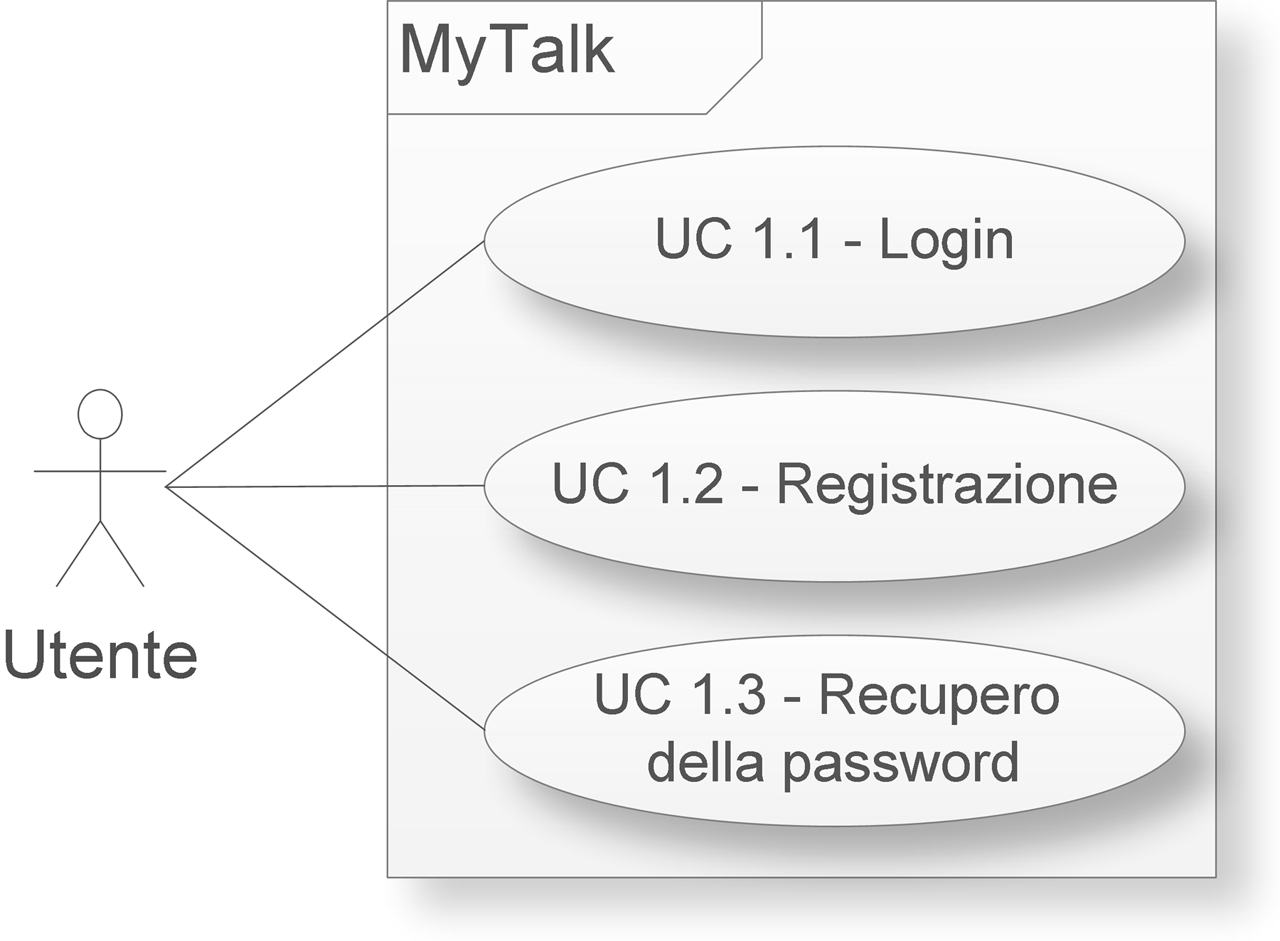
\includegraphics[width=.8\textwidth]{UC1}
\caption{UC1 - Login e registrazione}\label{fig:login_e_registrazione}
\end{center}
\end{figure}
\begin{description}
\item{\scshape\bfseries Attori principali:}Utente.
\item{\scshape\bfseries Scopo e descrizione:} L'utente può effettuare l'accesso al sistema mediante la procedura di autenticazione se registrato (UC1.1), recuperare la password dimenticata (UC1.3) oppure può provvedere alla propria registrazione (UC1.2), quindi effettuare successivamente l'accesso al sistema (UC1.1).
\item{\scshape\bfseries Precondizione:} Il sistema MyTalk è attivo e funzionante, le infrastrutture di rete sono attive.
\item{\scshape\bfseries Postcondizione:} L'utente si trova in uno di questi casi: ha avviato la procedura per l'autenticazione al sistema (UC1.1), oppure ha avviato la procedura per per la registrazione nel sistema (UC1.2), oppure ha avviato la procedura per il recupero della password dimenticata (UC1.3).
\item{\scshape\bfseries Illustrazione scenario principale:} L'utente può decidere di avviare la procedura di autenticazione al sistema (UC1.1), altrimenti se non ricorda le credenziali, può avviare la procedura per il recupero della password (UC1.3). Invece se l'utente sa di non essere registrato nel sistema, può avviare la procedura di registrazione (UC1.2).
\end{description}

\subsection{UC1.1: Login utente}
\begin{figure}[H]
\begin{center}
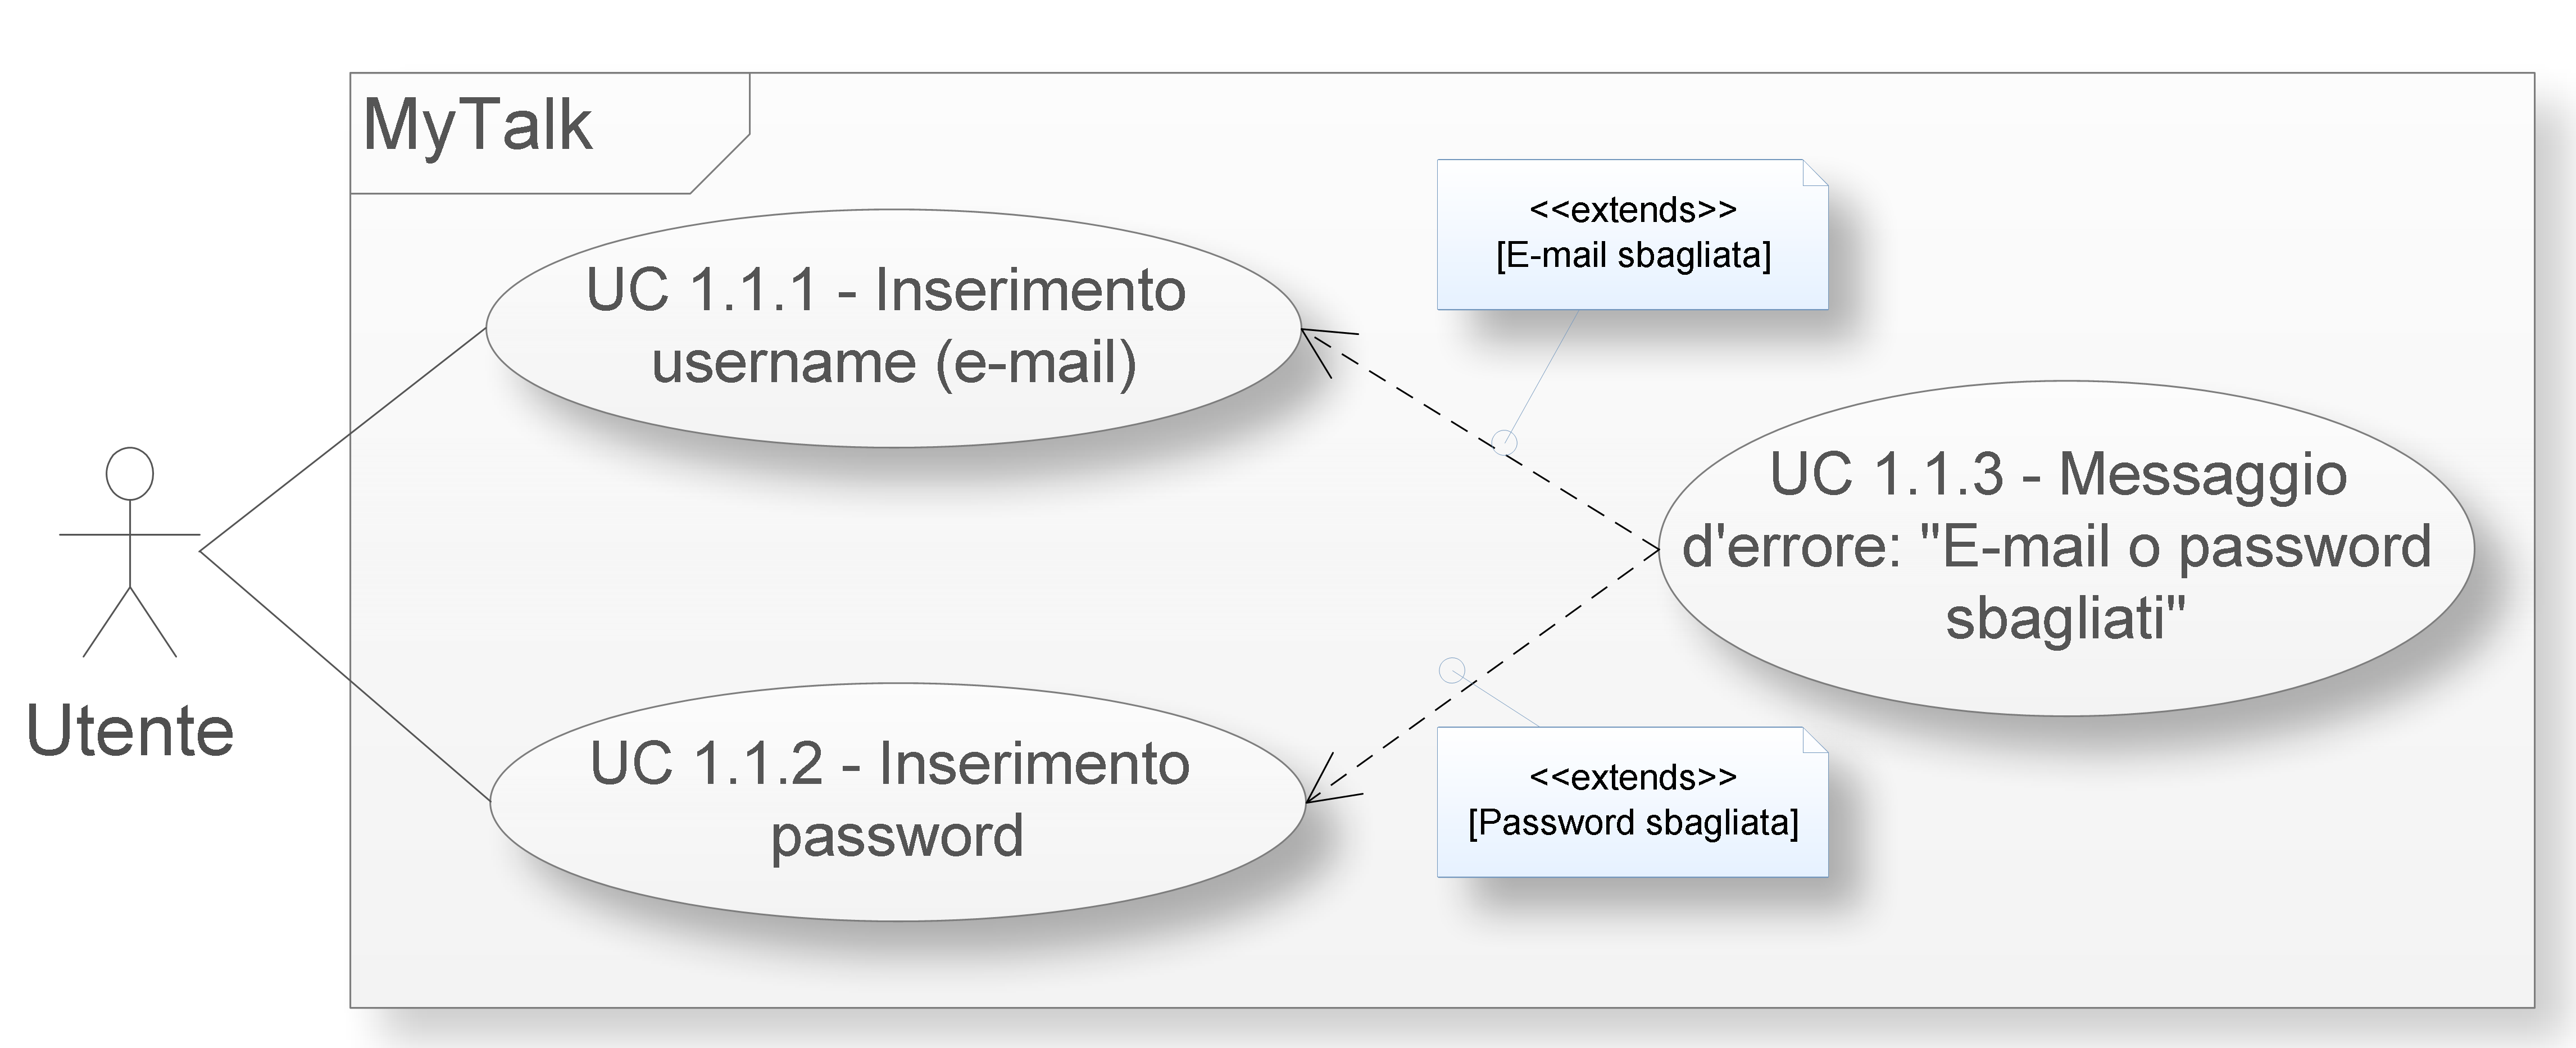
\includegraphics[width=.8\textwidth]{UC1-1}
\caption{UC1.1 - Login utente}\label{fig:login}
\end{center}
\end{figure}
\begin{description}
\item{\scshape\bfseries Attori principali:}Utente.
\item{\scshape\bfseries Scopo e descrizione:} L'utente si autentica per accedere al sistema MyTalk
\item{\scshape\bfseries Precondizione:} L'utente (generico) visualizza la schermata iniziale e il sistema è pronto.
\item{\scshape\bfseries Postcondizione:} L'utente è autenticato nel sistema
\item{\scshape\bfseries Illustrazione scenario principale:} L'utente inserisce username (UC1.1.1) e password (UC1.1.2) corretti e conferma.
\item{\scshape\bfseries Illustrazione scenario alternativo:} L'utente ha inserito dati non corretti: il sistema lo notifica con un errore unico (UC1.1.3) e rimane in attesa di una correzione. (Non vengono visualizzati due errori separati ma un errore unico generico per aumentare la sicurezza).
\end{description}

\subsection{UC1.2: Registrazione}
\begin{figure}[H]
\begin{center}
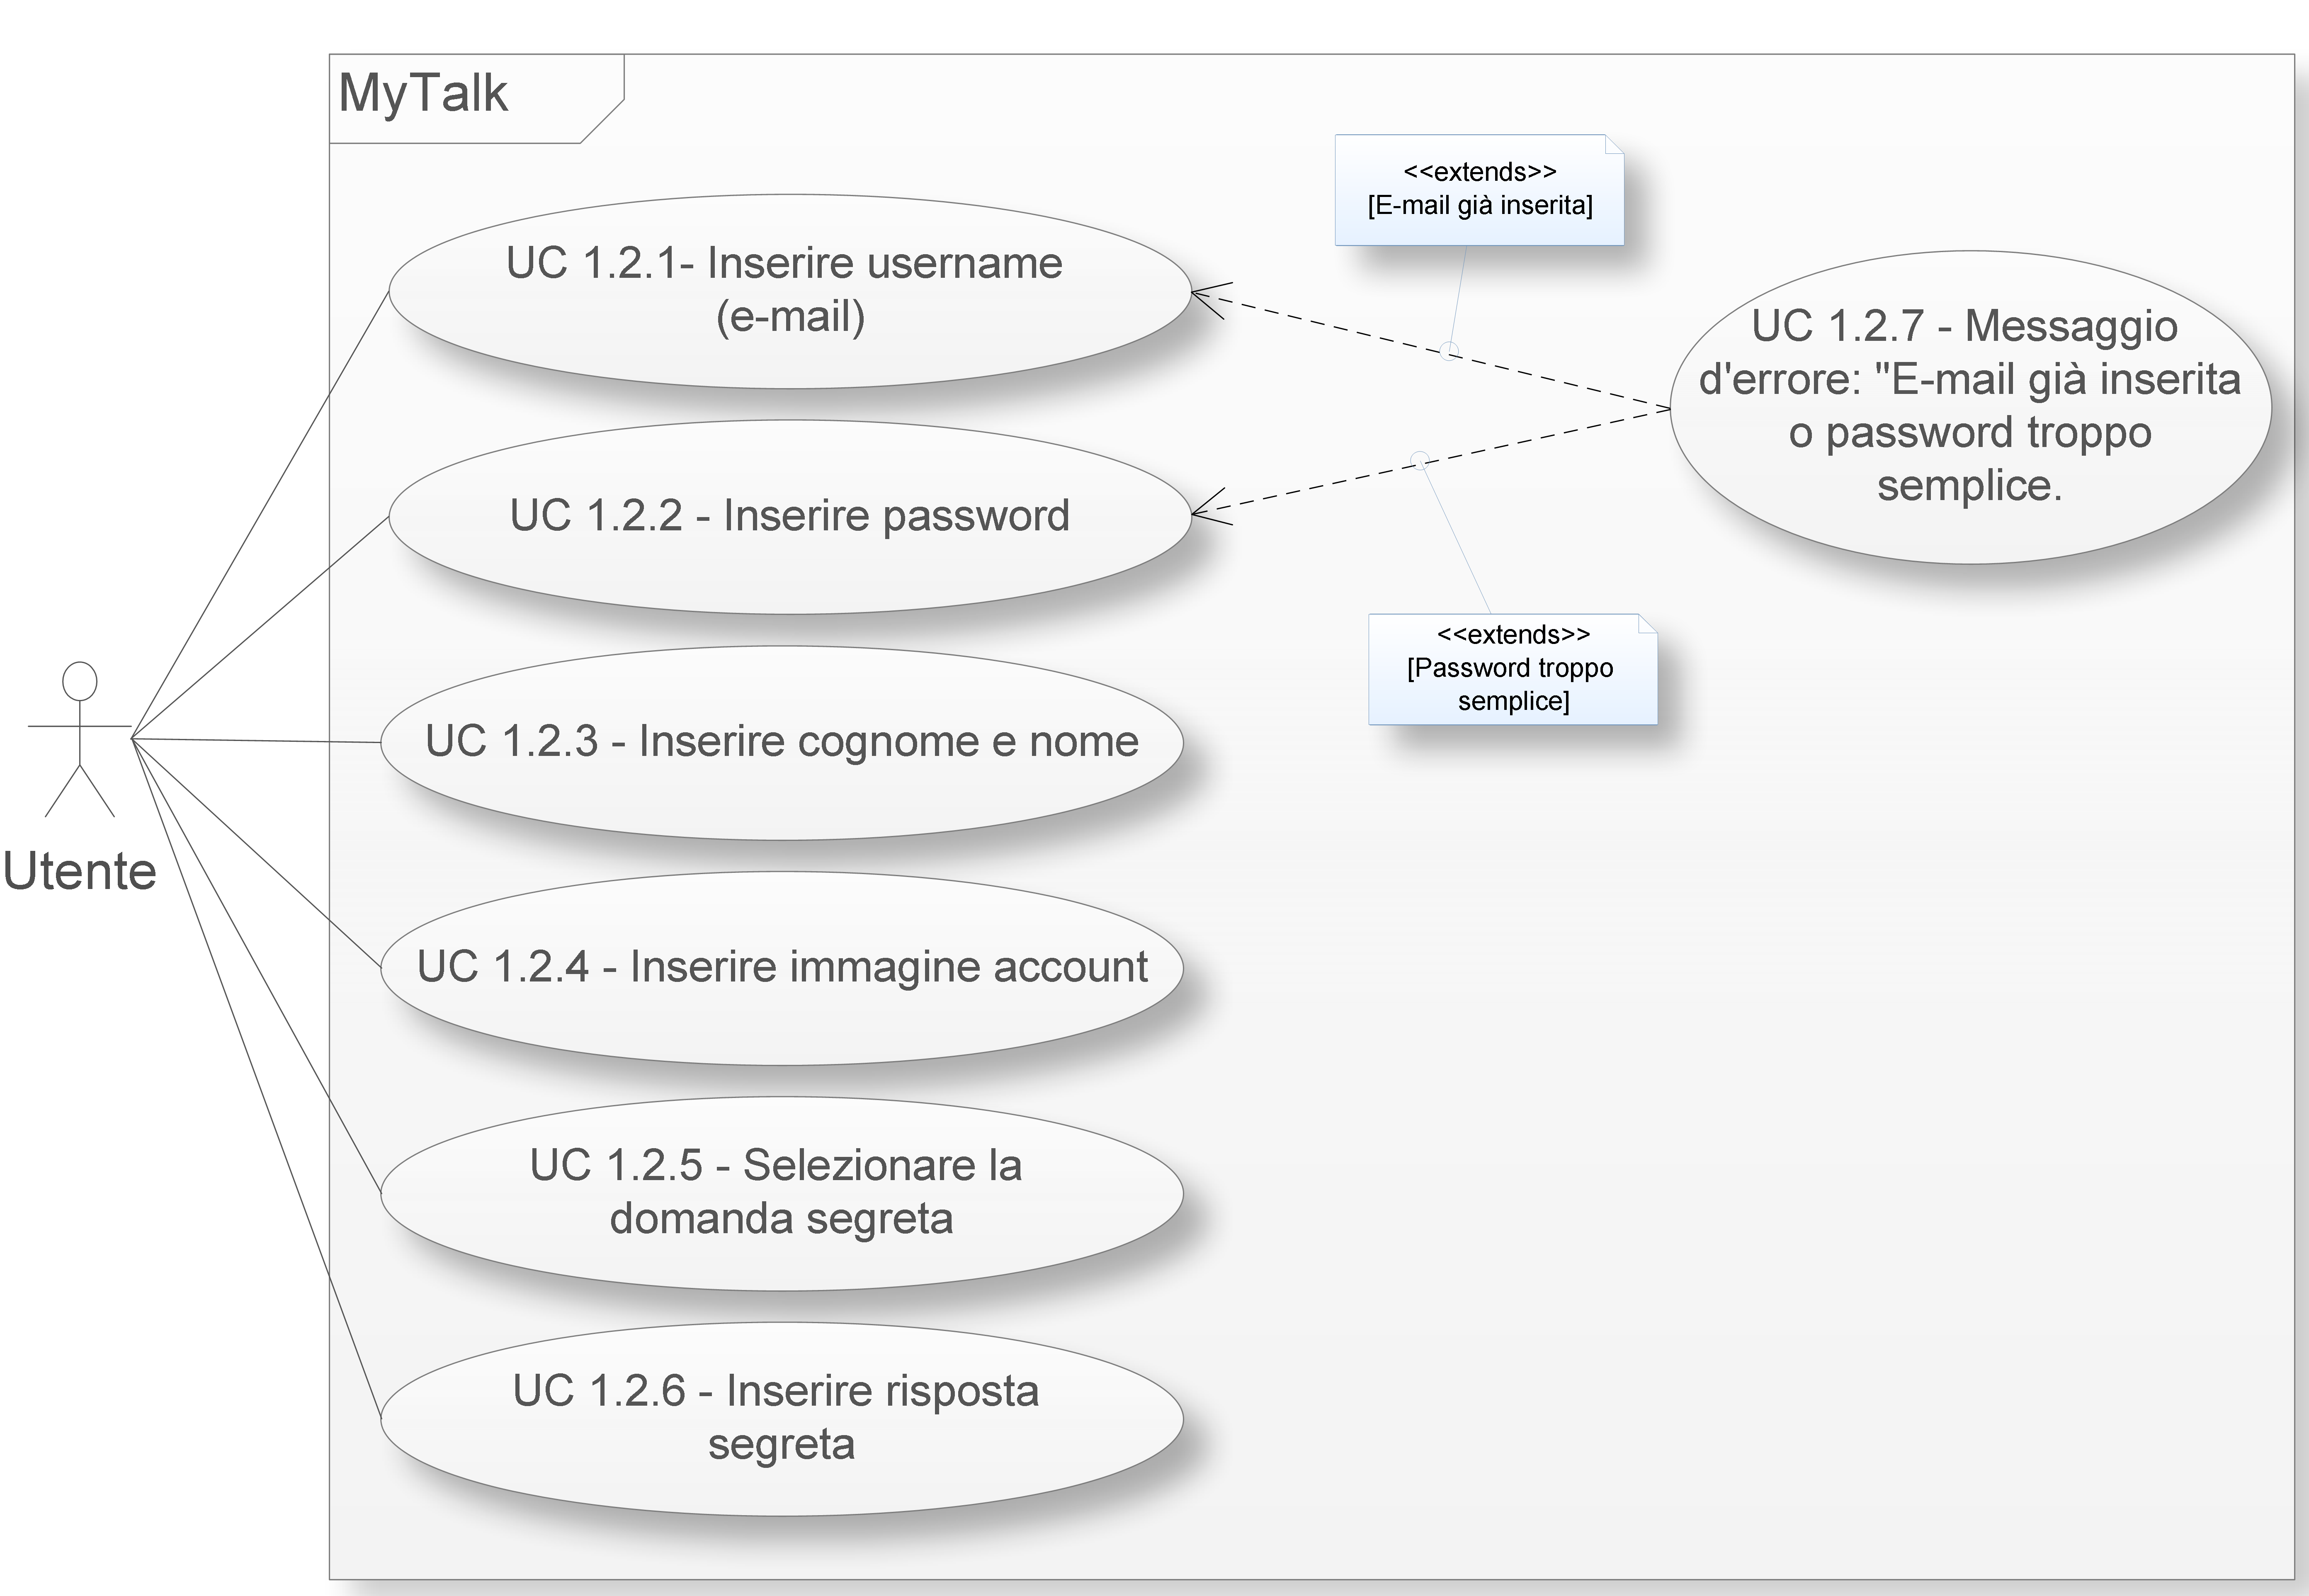
\includegraphics[width=.9\textwidth]{UC1-2}
\caption{UC1.2 - Registrazione}\label{fig:registrazione}
\end{center}
\end{figure}
\begin{description}
\item{\scshape\bfseries Attori principali:}Utente.
\item{\scshape\bfseries Scopo e descrizione:} L'utente si registra nel sistema.
\item{\scshape\bfseries Precondizione:} L'utente (generico) visualizza la schermata iniziale e il sistema è pronto.
\item{\scshape\bfseries Postcondizione:} L'utente si è registrato nel sistema MyTalk
\item{\scshape\bfseries Illustrazione scenario principale:} La registrazione di un nuovo account comporta l'inserimento di un indirizzo email come ID utente (UC1.2.1), una password (UC1.2.2), domanda segreta (UC1.2.6) e la relativa risposta (UC1.2.7). Il nome (UC1.2.3), il cognome (UC1.2.4) e un'immagine (UC1.2.5) da associare al proprio profilo possono essere inserite facoltativamente. Per andare a buon fine la procedura di registrazione richiede che la password prescelta assicuri un sufficiente livello di complessità e prevede altresì la selezione della domanda segreta (e della relativa risposta) necessarie al recupero della password in caso di smarrimento, nonché la validazione dell''indirizzo email al fine di verificare che l''utente ne sia effettivamente in possesso.
\item{\scshape\bfseries Illustrazione scenario alternativo:} Il sistema può fallire per via dell'inserimento di dati non corretti. Il sistema mostra un errore relativo all'username (UC1.2.8) oppure alla password (UC1.2.9)
\end{description}

\subsection{UC1.3: Recupero della password}
\begin{figure}[H]
\begin{center}
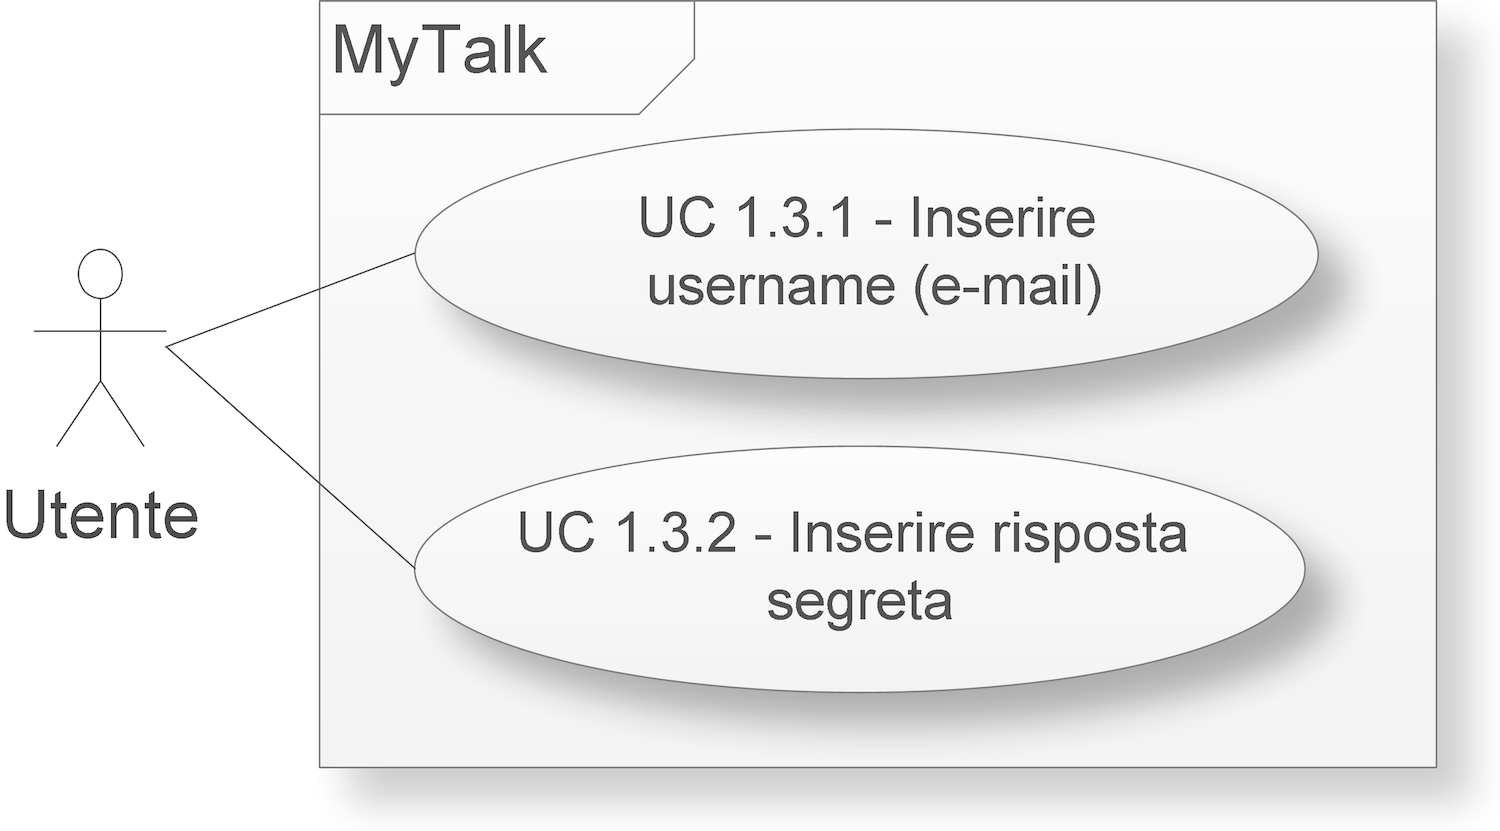
\includegraphics[width=.8\textwidth]{UC1-3}
\caption{UC1.3 - Recupero della password}\label{fig:recupero}
\end{center}
\end{figure}
\begin{description}
\item{\scshape\bfseries Attori principali:}Utente.
\item{\scshape\bfseries Scopo e descrizione:} L'utente desidera recuperare la password smarrita.
\item{\scshape\bfseries Precondizione:} L'utente (generico) visualizza la schermata iniziale e il sistema è pronto.
\item{\scshape\bfseries Postcondizione:} L'utente riceve per e-mail la password dimenticata.
\item{\scshape\bfseries Illustrazione scenario principale:} Si avvia la procedura di recupero della password: l'utente deve inserire l'e-mail (UC1.3.1) e la risposta alla domanda segreta (UC1.3.2). A questo segue l'invio della password all'indirizzo email indicato in fase di registrazione.
\item{\scshape\bfseries Illustrazione scenario alternativo:} Il sistema può fallire per via dell'inserimento di dati non corretti. Il sistema evidenzia gli errori e rimane in attesa della correzione.
\end{description}

\subsection{UC2: Home screen dell'applicativo}
\begin{figure}[H]
\begin{center}
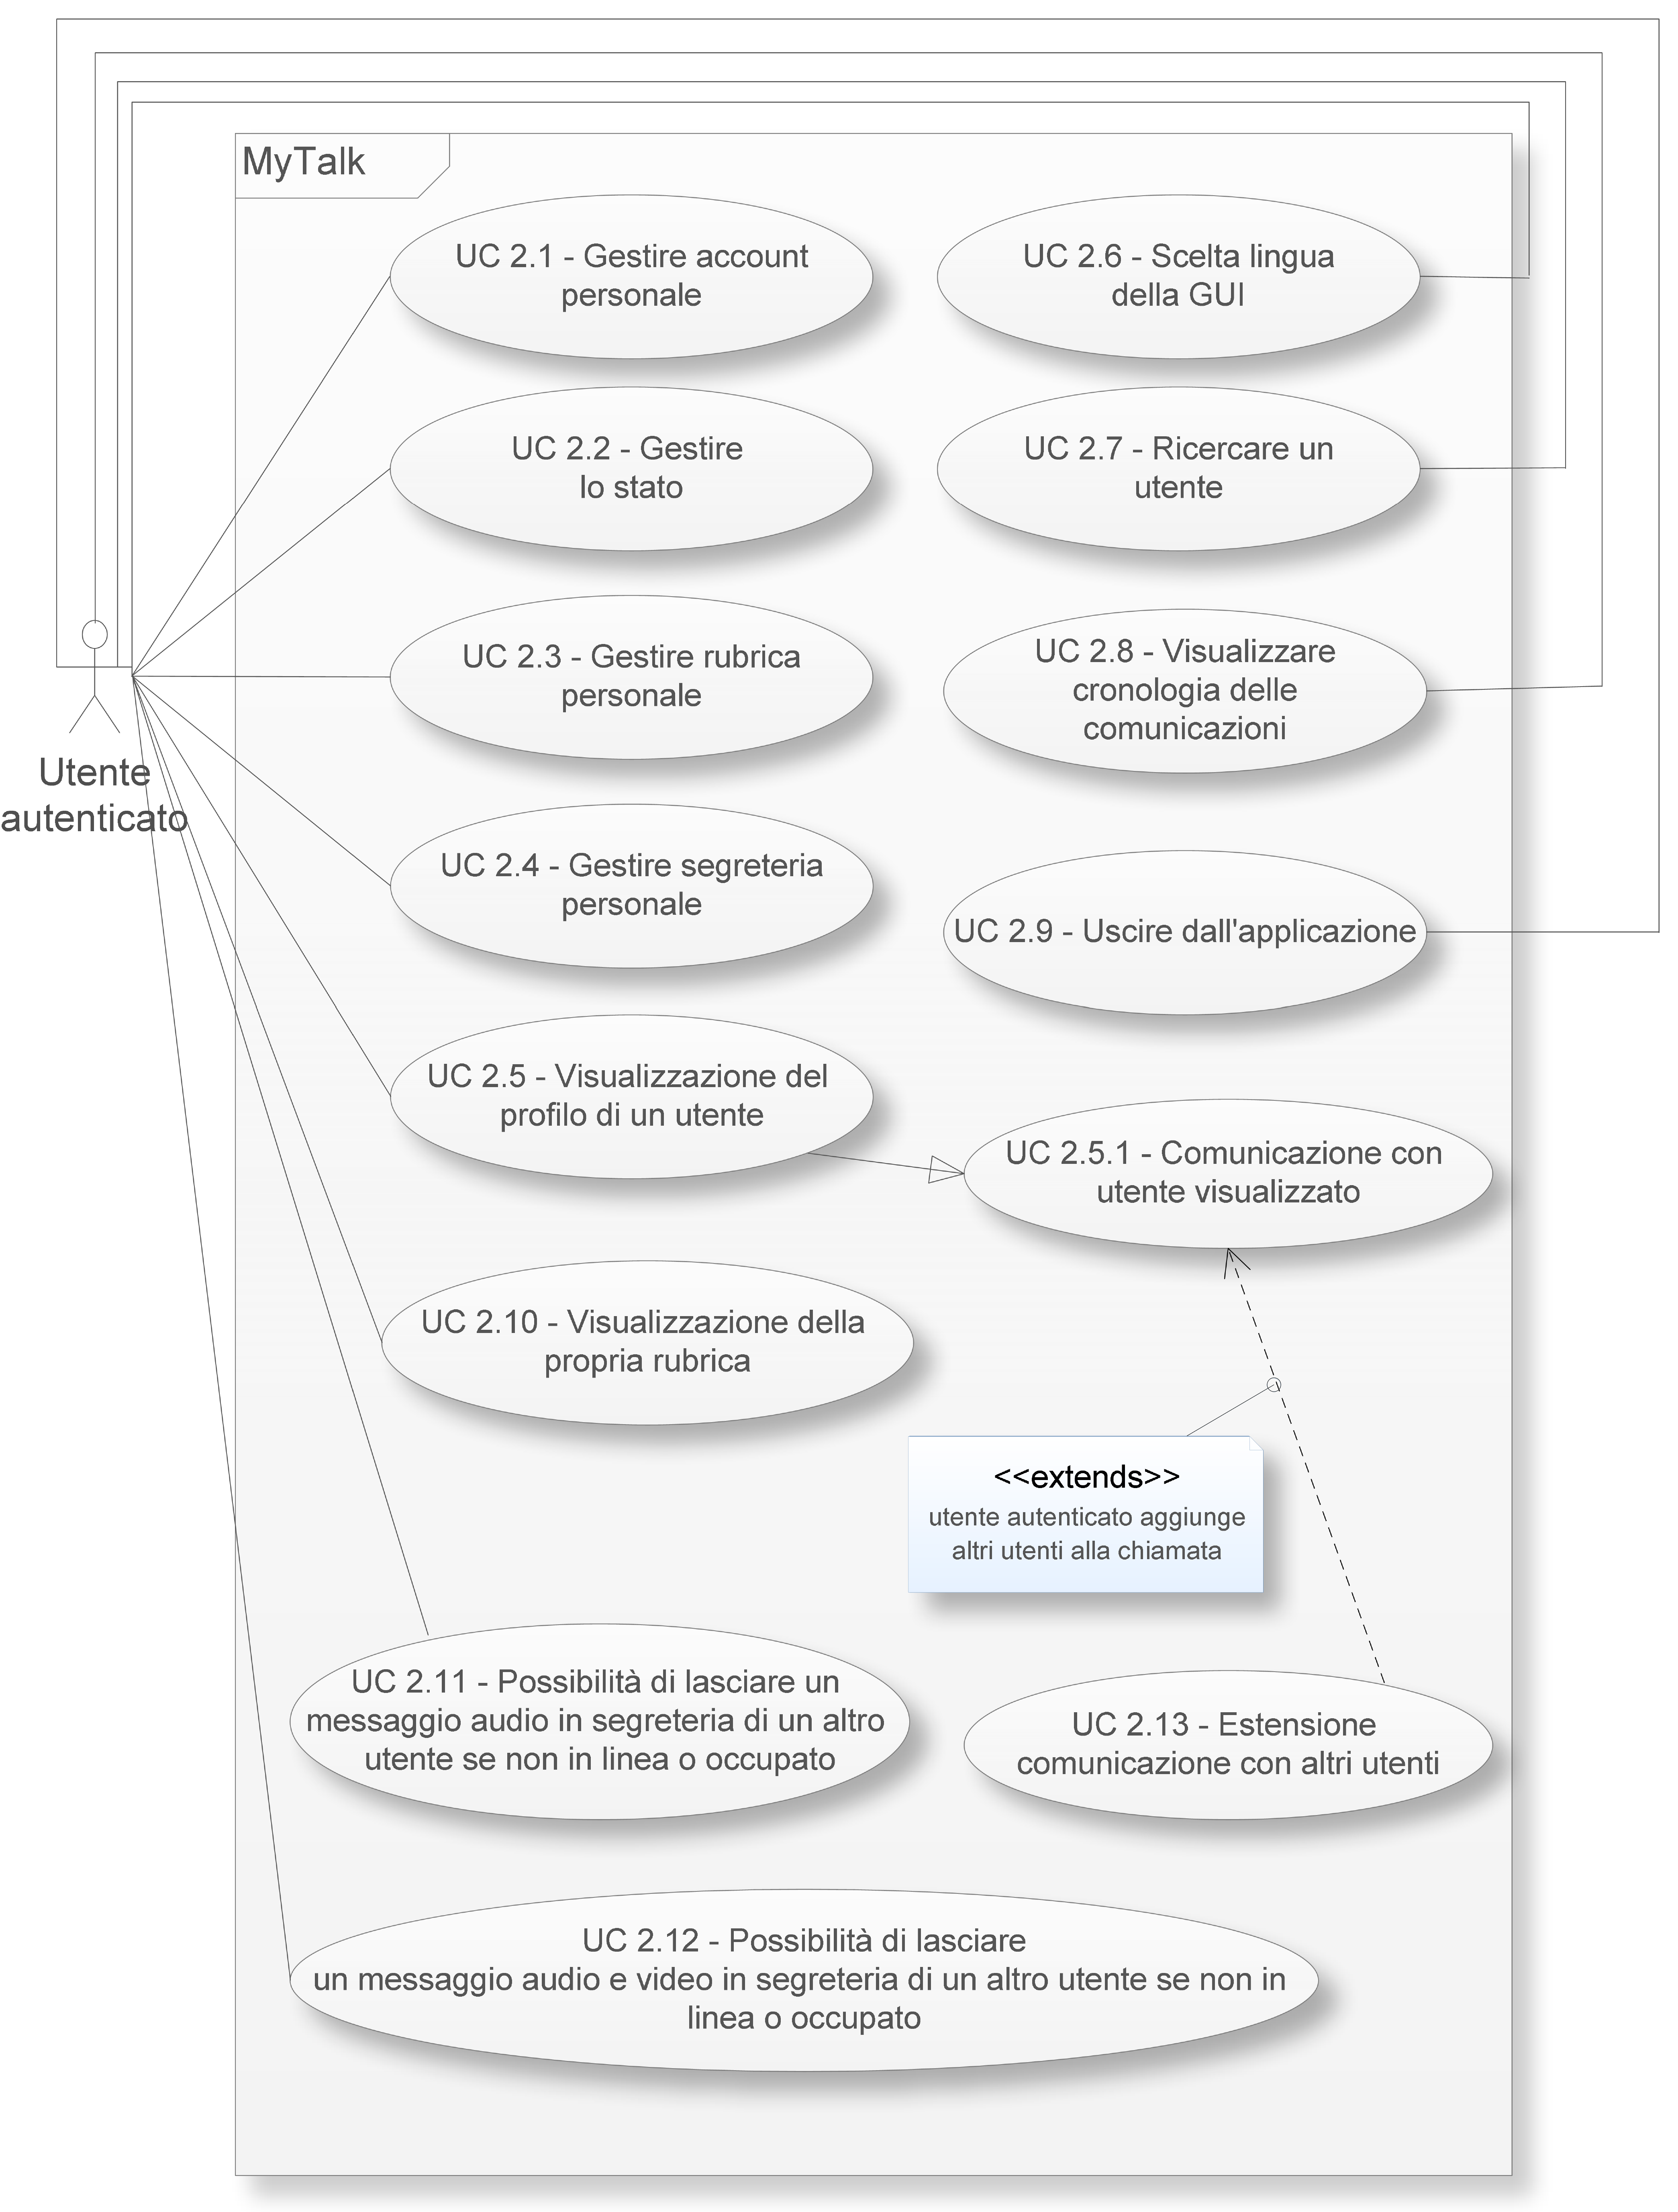
\includegraphics[width=.8\textwidth]{UC2}
\caption{UC2 - Home screen dell'applicativo}\label{fig:home}
\end{center}
\end{figure}
\begin{description}
\item{\scshape\bfseries Attori principali:}Utente autenticato.
\item{\scshape\bfseries Scopo e descrizione:} Funzionalità generali offerte all'utente autenticato e presenti nella Home screen dell'applicativo.
\item{\scshape\bfseries Precondizione:} L'utente ha effettuato il login ed è autenticato nel sistema.
\item{\scshape\bfseries Postcondizione:} L'utente ha eseguito una delle funzioni proposte.
\item{\scshape\bfseries Illustrazione scenario principale:} L'utente dopo aver eseguito il login al sistema, si trova nella Home dell'applicativo. Qui può svolgere una delle seguenti opzioni: gestire il proprio account (UC2.1), scegliere la lingua della GUI (UC2.6), gestire lo stato (UC2.2), eseguire delle ricerche di utenti (UC2.7), gestire la propria rubrica (UC2.3), lasciare un messaggio nella segreteria di un utente (UC2.13 - UC2.14), gestire la propria segreteria (UC2.4), visualizzare la cronologia delle comunicazioni (UC2.9), stabilire connessioni con altri utenti (UC2.5) e  visualizzare gli utenti registrati nel sistema  (UC2.10). Infine l'utente ha la possibilità di chiudere l'applicativo (UC2.11).
\item{\scshape\bfseries Illustrazione scenario alternativo:} L'utente, se ha già avviato una connessione con un altro utente, può estenderla con altri (UC2.12).
\end{description}

\subsection{UC2.1: Gestione account}
\begin{figure}[H]
\begin{center}
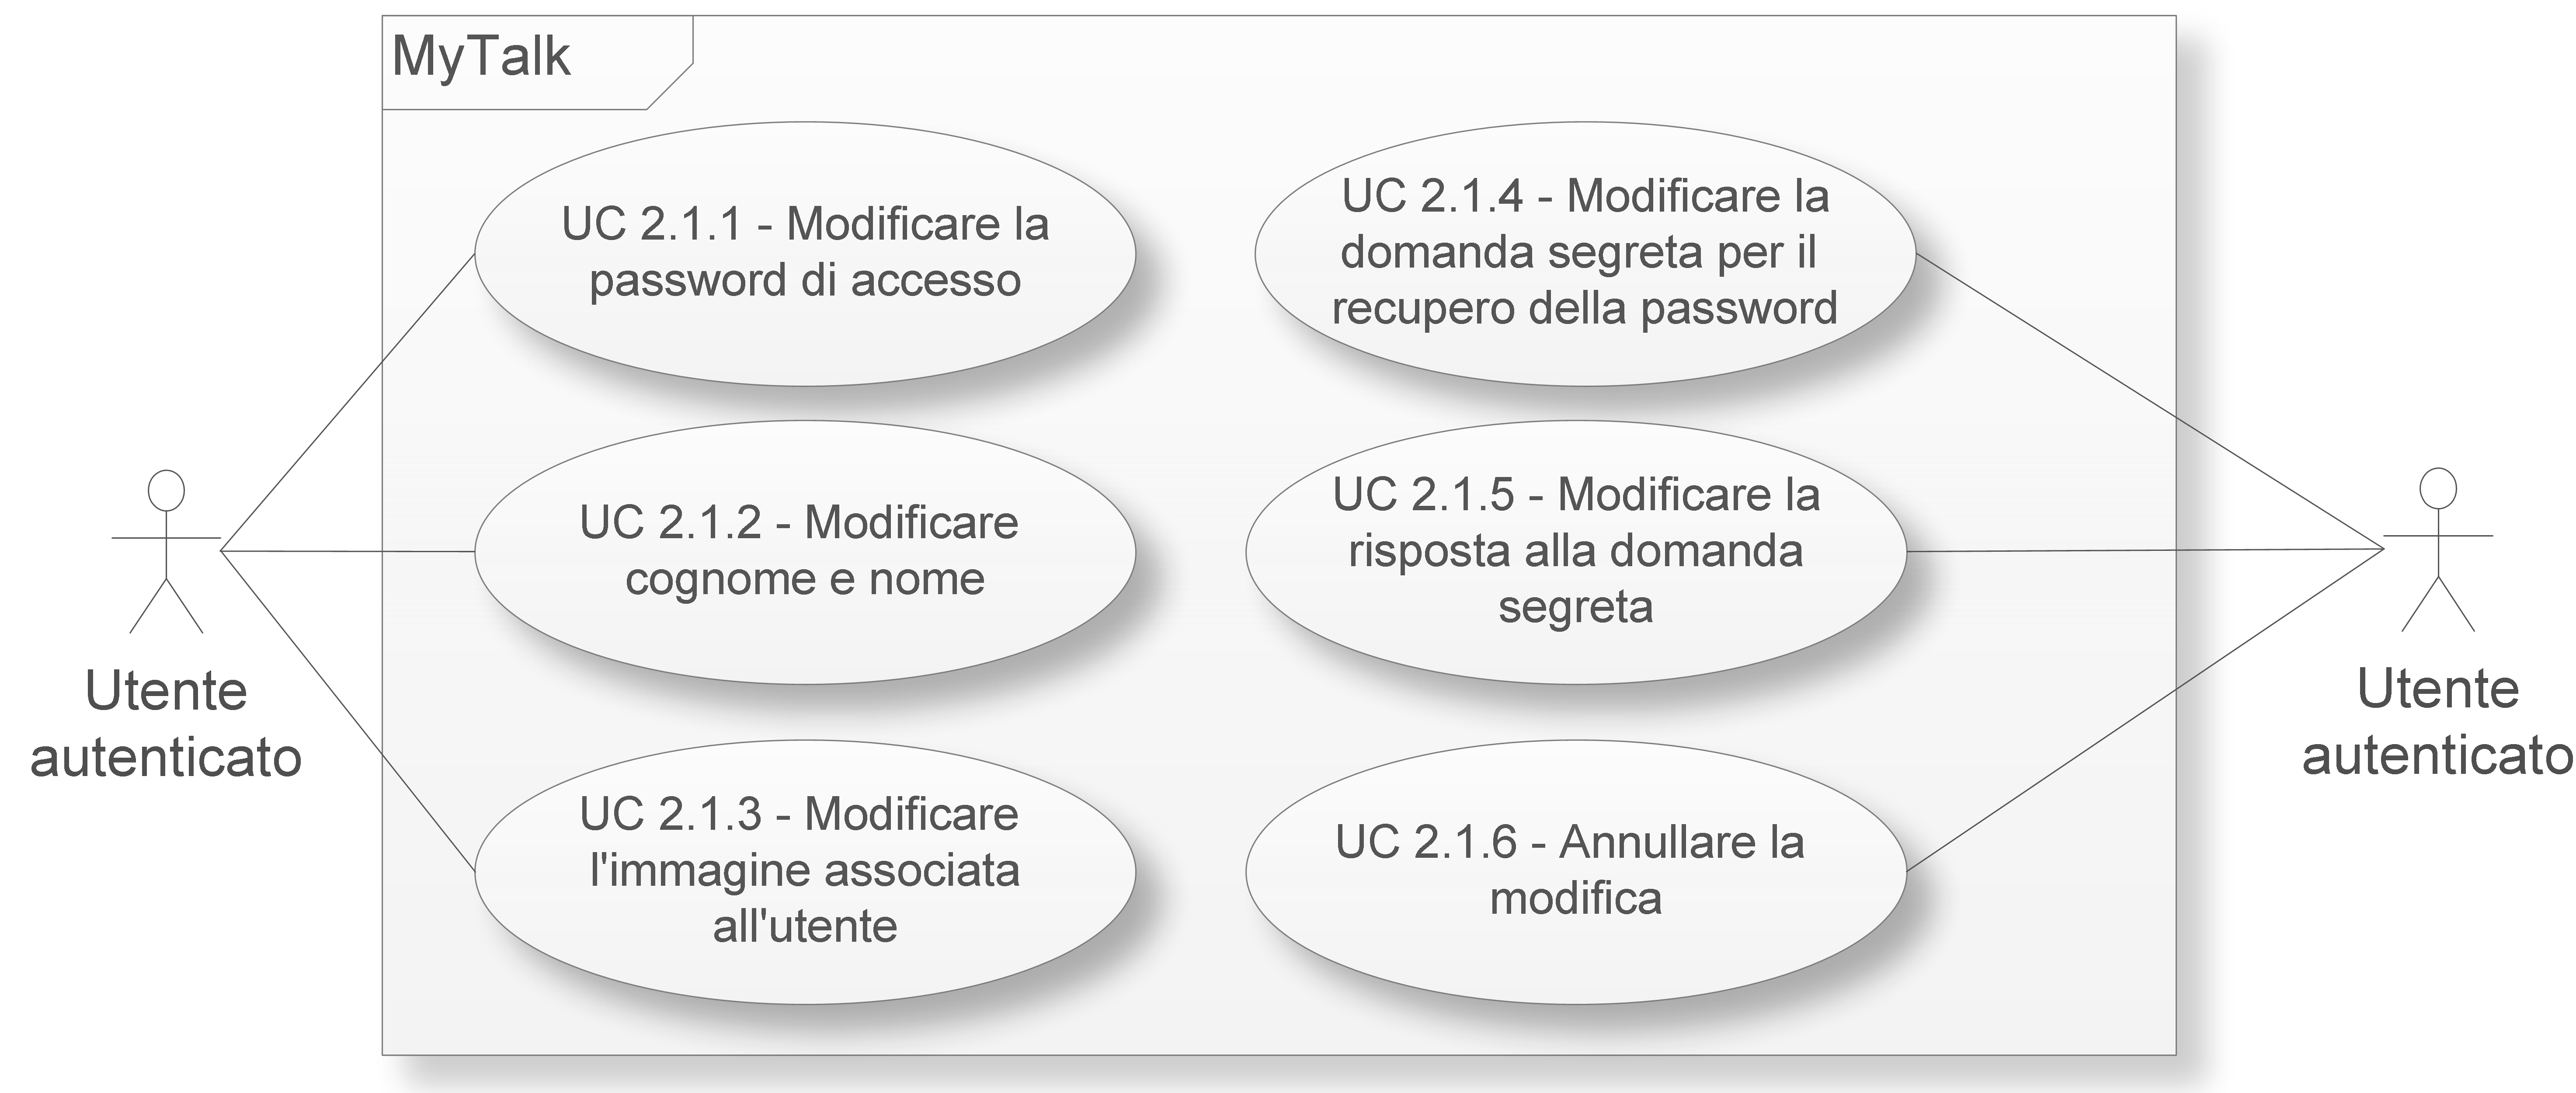
\includegraphics[width=.8\textwidth]{UC2-1}
\caption{UC2.1: Gestione account}\label{fig:gestione_account}
\end{center}
\end{figure}
\begin{description}
\item{\scshape\bfseries Attori principali:}Utente autenticato.
\item{\scshape\bfseries Scopo e descrizione:} un utente autenticato, ha la possibilità di modificare i propri dati personali, inseriti durante la sua registrazione, così da rimediare ad eventuali errori.
\item{\scshape\bfseries Precondizione:} l'utente corrente e' registrato nel sistema, ed ha effettuato il login.
\item{\scshape\bfseries Postcondizione:} i dati dell'utente sono stati aggiornati con i valori da lui inseriti.
\item{\scshape\bfseries Illustrazione scenario principale:} L'utente visualizza i valori correnti dei dati che lo riguardano e può apportare
le modifiche che ritiene necessarie. I dati che può modificare sono la password (UC2.1.1), il nome (UC2.1.2), il cognome (UC2.1.6), l'immagine profilo (UC2.1.3), la domanda segreta (UC2.1.4), la risposta alla domanda segreta (UC2.1.5). A questo punto può salvare le modifiche (UC2.1.8).
\item{\scshape\bfseries Illustrazione scenario alternativo:} Prima del salvataggio (UC2.1.8) l'utente può annullare l'operazione (UC2.1.7) tornando così alla schermata principale senza aver effettuato nessuna modifica.
\end{description}

\subsection{UC2.2: Gestire lo stato}
\begin{figure}[H]
\begin{center}
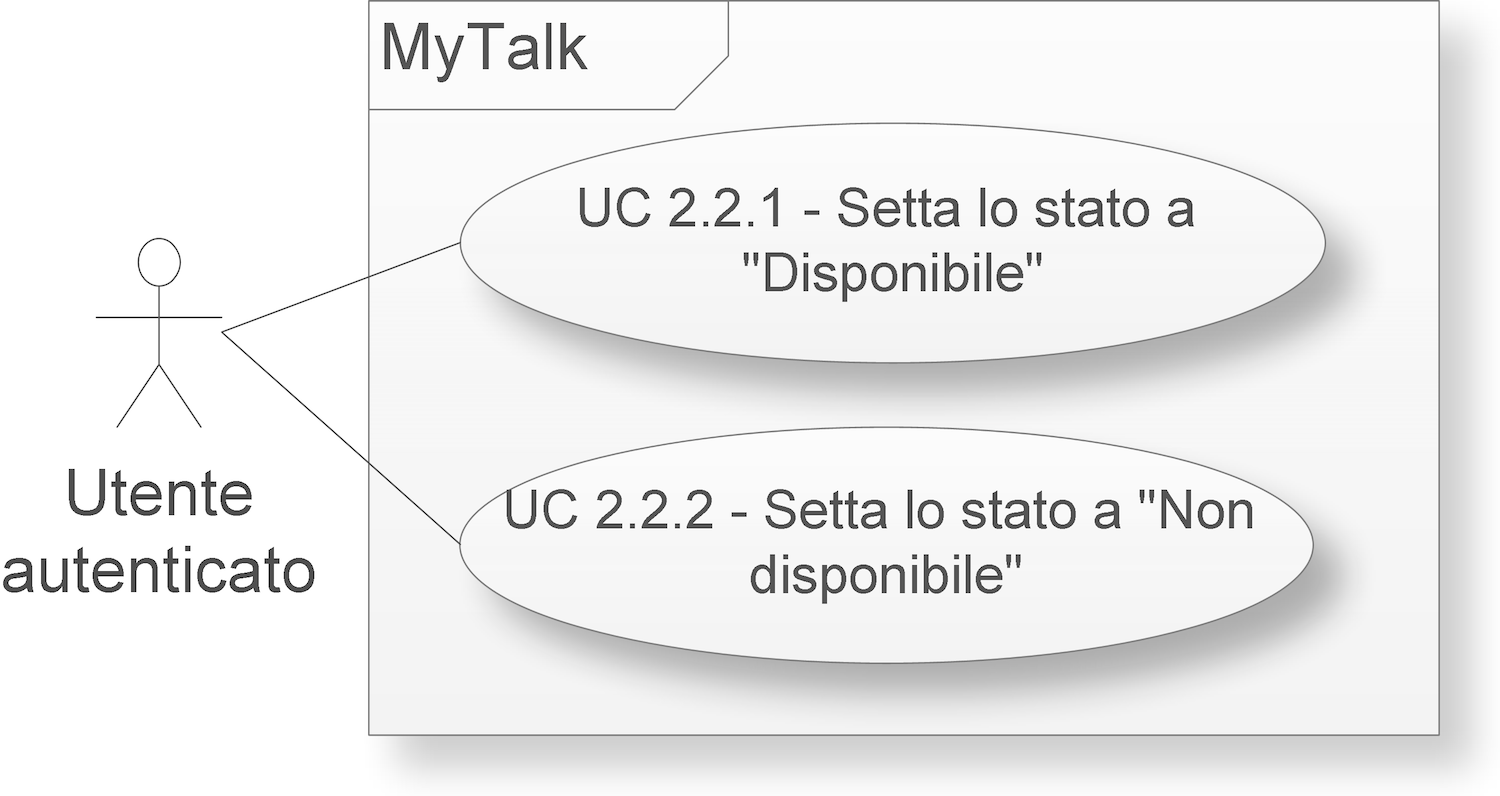
\includegraphics[width=.8\textwidth]{UC2-2}
\caption{UC2.2: Gestire lo stato utente}\label{fig:gestione_stato}
\end{center}
\end{figure}
\begin{description}
\item{\scshape\bfseries Attori principali:}Utente autenticato.
\item{\scshape\bfseries Scopo e descrizione:} L'utente potrà comunicare agli altri utenti la sua disponibilità o meno a comunicare, aggiornando il proprio stato.
\item{\scshape\bfseries Precondizione:} L'utente è registrato nel sistema ed ha eseguito l'accesso senza errori.
\item{\scshape\bfseries Postcondizione:} L'utente ha modificato il proprio stato.
\item{\scshape\bfseries Illustrazione scenario principale:} L'utente potrà scegliere di cambiare il proprio stato corrente. Gli stati tra cui può scegliere sono:disponibile (UC2.2.1)  e non disponibile (UC2.2.2).
\end{description}

\subsection{UC2.3: Gestione della rubrica}
\begin{figure}[[h!]]
\begin{center}
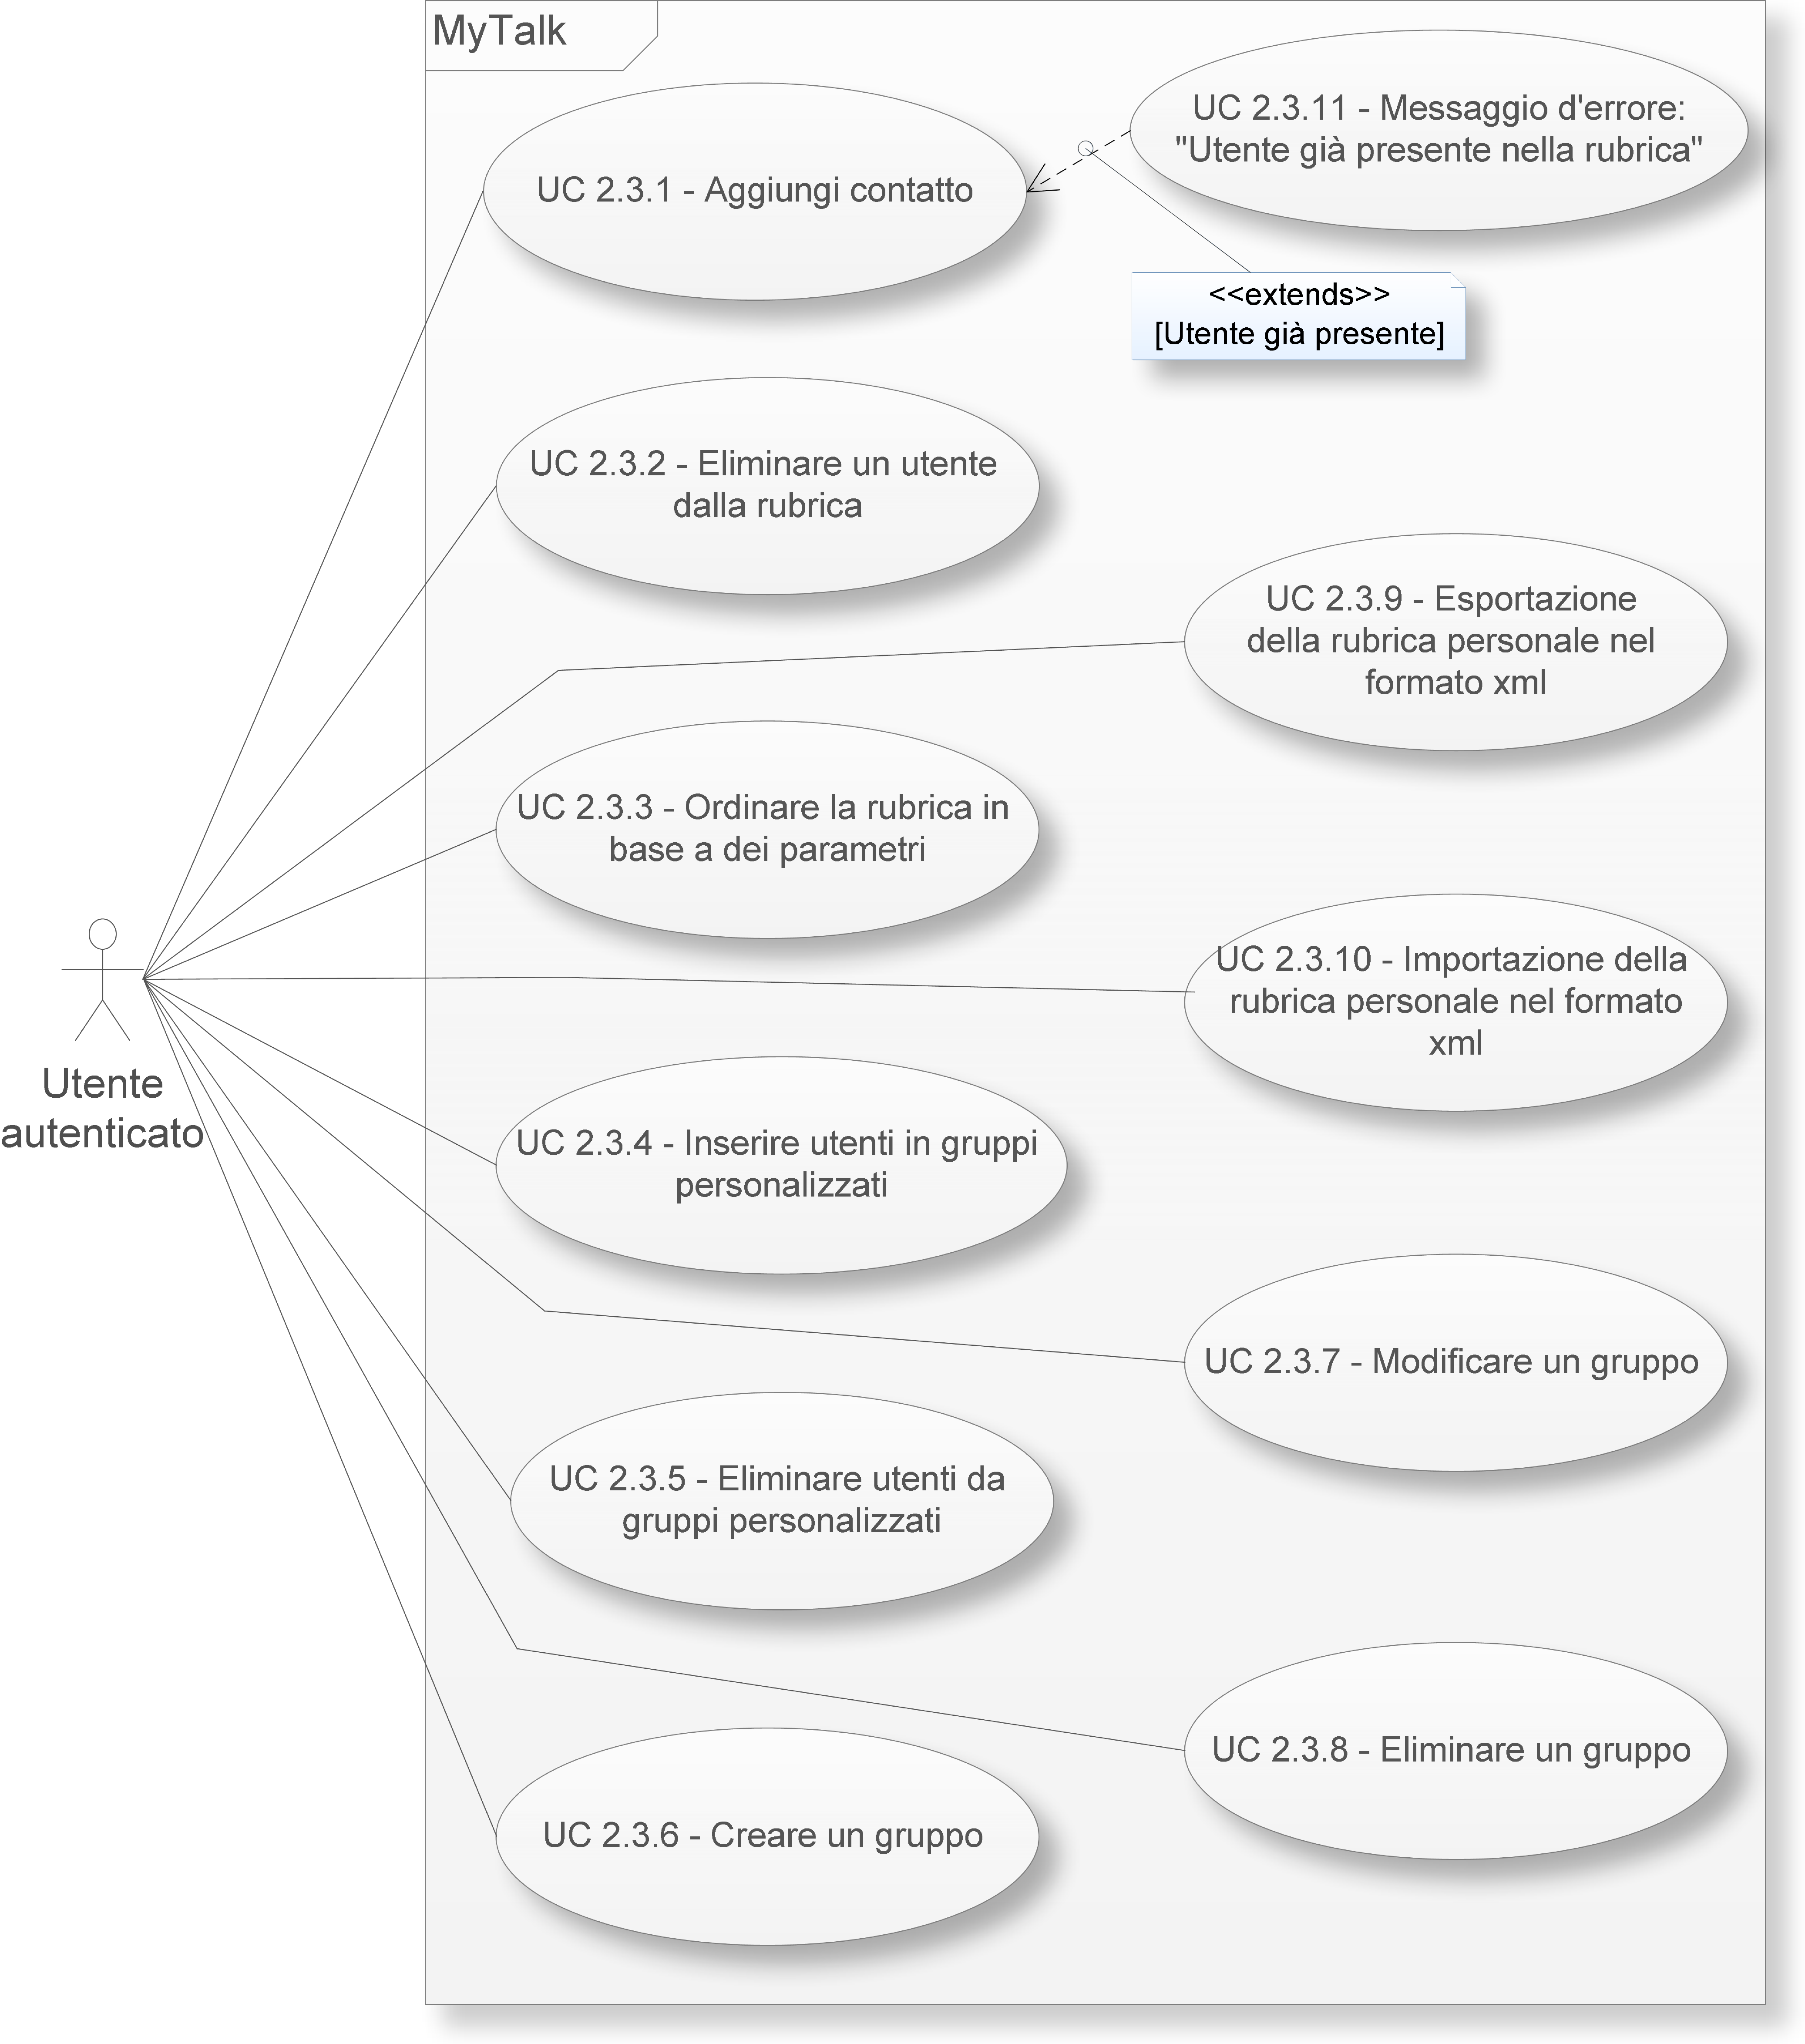
\includegraphics[width=.8\textwidth]{UC2-3}
\caption{UC2.3: Gestione della rubrica}\label{fig:gestione_rubrica}
\end{center}
\end{figure}
\begin{description}
\item{\scshape\bfseries Attori principali:}Utente autenticato.
\item{\scshape\bfseries Scopo e descrizione:} L'utente può visualizzare ed organizzare la rubrica dei propri contatti personali sulla base della lista degli utenti che si sono registrati, oppure importando i contati da un file esterno.
\item{\scshape\bfseries Precondizione:} L'utente ha effettuato la procedura di login ed è quindi autenticato.
\item{\scshape\bfseries Postcondizione:} Se l'utente ha attuato delle modifiche, queste sono state salvate. Altrimenti non ci sono state modifiche sui dati inerenti la rubrica.
\item{\scshape\bfseries Illustrazione scenario principale:} L'utente visualizza la lista di utenti registrati nel sistema, affiancata dalla propria rubrica divisa in gruppi. Quindi può scegliere una delle seguenti opzioni: aggiunge un contatto alla rubrica (UC2.3.1), aggiunge un contatto alla rubrica black-list (UC2.3.4), crea un nuovo gruppo (UC2.3.6); elimina un gruppo (UC2.3.8), aggiunge ed eliminare un contatto alla rubrica in un gruppo scelto tra quelli già creati (UC2.3.4 - UC2.3.5), elimina un contatto dalla propria rubrica (UC2.3.2), esporta i contatti presenti nella propria rubrica (UC2.3.9) e importa dei contatti prelevati da un file XML (UC2.3.10).
Inoltre potrà ordinare la rubrica in base a dei parametri (UC2.3.3) e ricercare un utente nella rubrica (UC2.3.11).
\end{description}

\subsection{UC2.3.1: Aggiungi contatto}
\begin{figure}[H]
\begin{center}
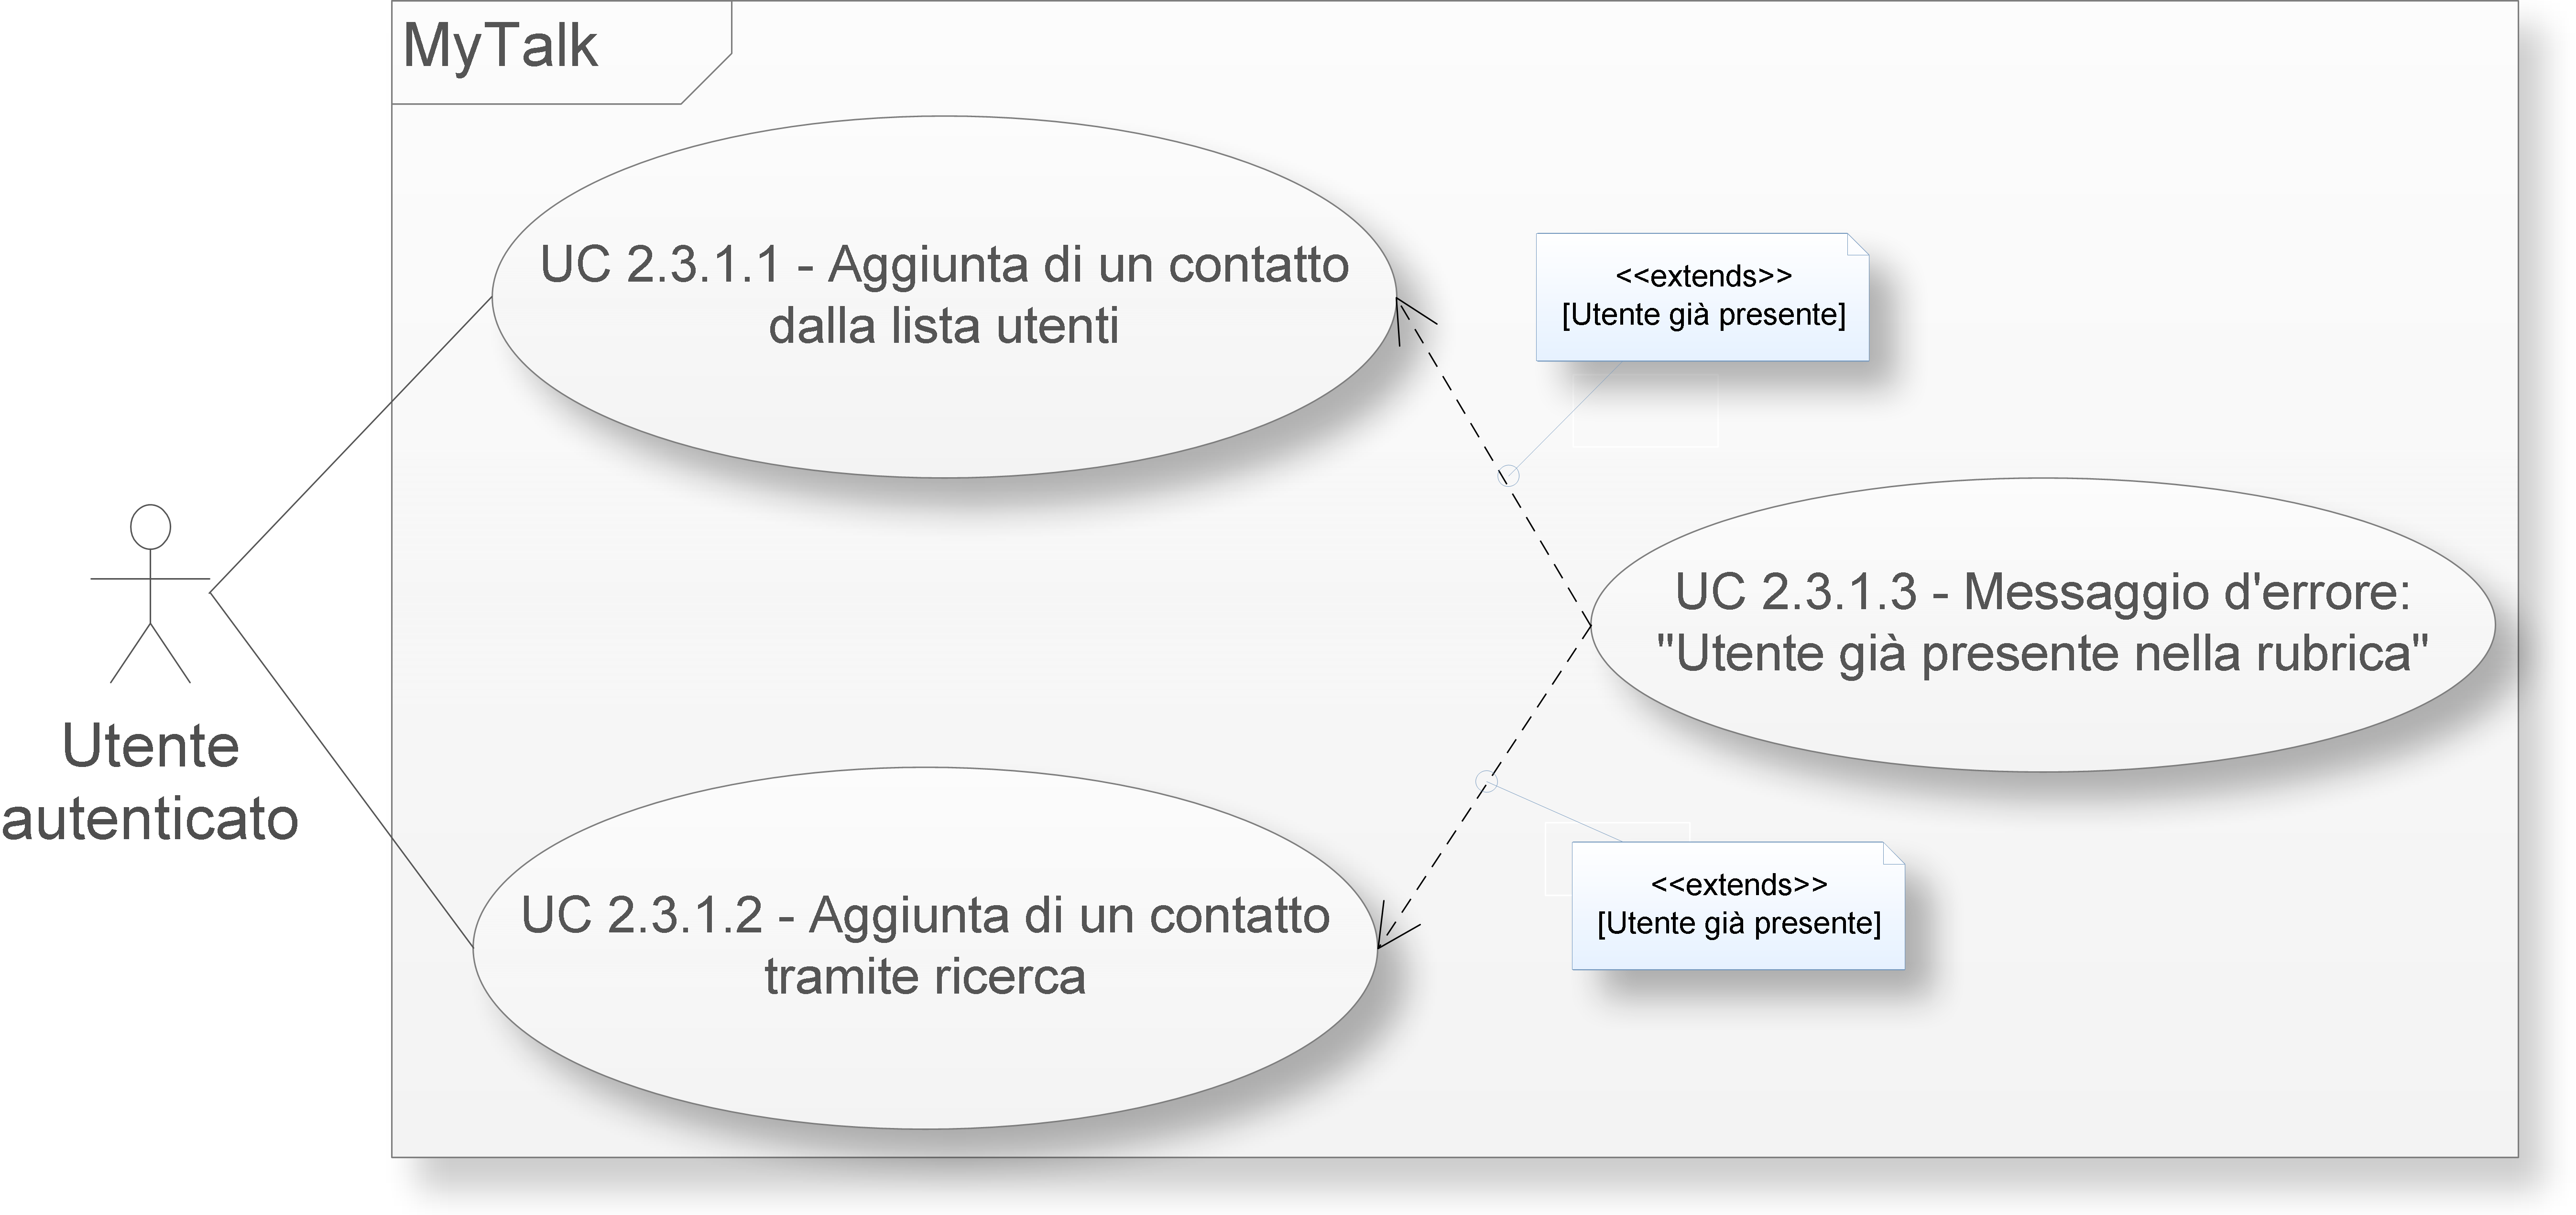
\includegraphics[width=.9\textwidth]{UC2-3-1}
\caption{UC2.3.1: Aggiungi contatto}\label{fig:aggiungi_contatto}
\end{center}
\end{figure}
\begin{description}
\item{\scshape\bfseries Attori principali:}Utente autenticato.
\item{\scshape\bfseries Scopo e descrizione:} L'utente aggiunge un contatto alla propria rubrica.
\item{\scshape\bfseries Precondizione:} L'utente e' autenticato al sistema; la lista degli utenti registrati presso il server non è vuota.
\item{\scshape\bfseries Postcondizione:} L'utente ha aggiunto un nuovo contatto nella propria rubrica.
\item{\scshape\bfseries Illustrazione scenario principale:} L'utente può operare l'inserimento seguendo 2 iter. Nel primo caso l'utente seleziona un contatto direttamente dalla lista degli iscritti (UC2.3.1.1). Nel secondo caso l'utente cerca un contatto per aggiungerlo (UC2.3.1.2).
\item{\scshape\bfseries Illustrazione scenario alternativo:} Se la ricerca del contatto da esito negativo viene riportato un errore (UC2.3.1.3).
\item{\scshape\bfseries Illustrazione scenario alternativo:} Se il contatto selezionato per l'inserimento nella rubrica, è già presente nella rubrica, allora compare un messaggio d'errore (UC2.3.1.3) che avvisa l'utente dell'inpossibilità di aggiungere il contatto. (Non vengono visualizzati due errori separati ma un errore unico).
\end{description}

\subsection{UC2.4: Gestire segreteria personale}
\begin{figure}[H]
\begin{center}
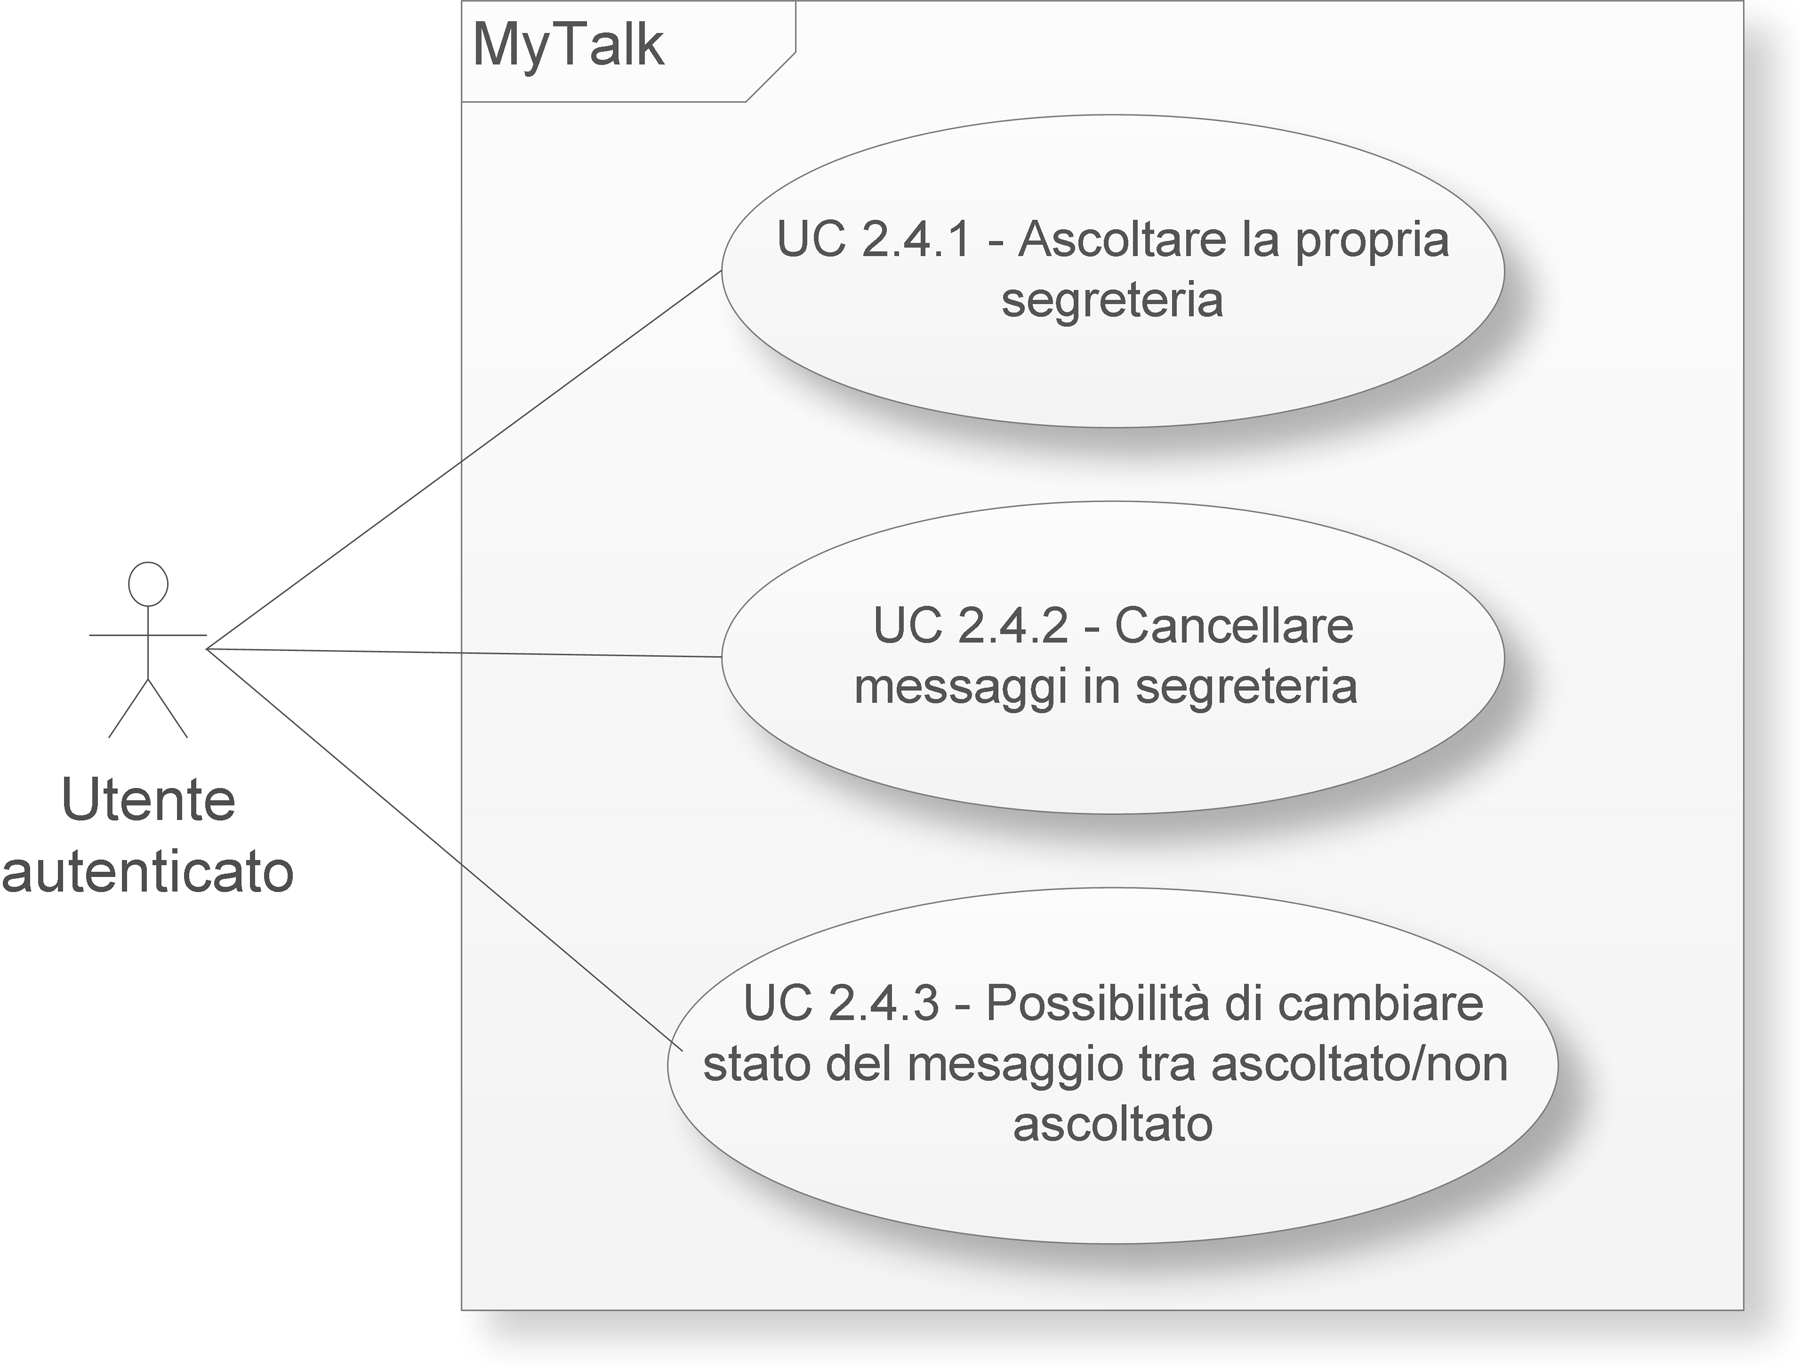
\includegraphics[width=.8\textwidth]{UC2-4}
\caption{UC2.4: Gestire segreteria personale}\label{fig:segreteria}
\end{center}
\end{figure}
\begin{description}
\item{\scshape\bfseries Attori principali:}Utente autenticato.
\item{\scshape\bfseries Scopo e descrizione:} L'utente ha a disposizione una segreteria personale che può gestire.
\item{\scshape\bfseries Precondizione:} L'utente ha effettuato la procedura di login ed è quindi autenticato.
\item{\scshape\bfseries Postcondizione:} Il sistema ha eseguito con successo le operazioni richieste dall'utente.
\item{\scshape\bfseries Illustrazione scenario principale:} L'utente si trova nella sezione riguardante la segreteria e può ascoltare, se presenti, i messaggi lasciati dai propri contatti (UC2.4.1), cancellarle i messaggi ricevuti (UC2.4.2) ed infine cambiare lo stato del messaggio da letto a da leggere e viceversa.
\end{description}

\subsection{UC2.5: Connessione con altri utenti autenticati}
\begin{figure}[H]
\begin{center}
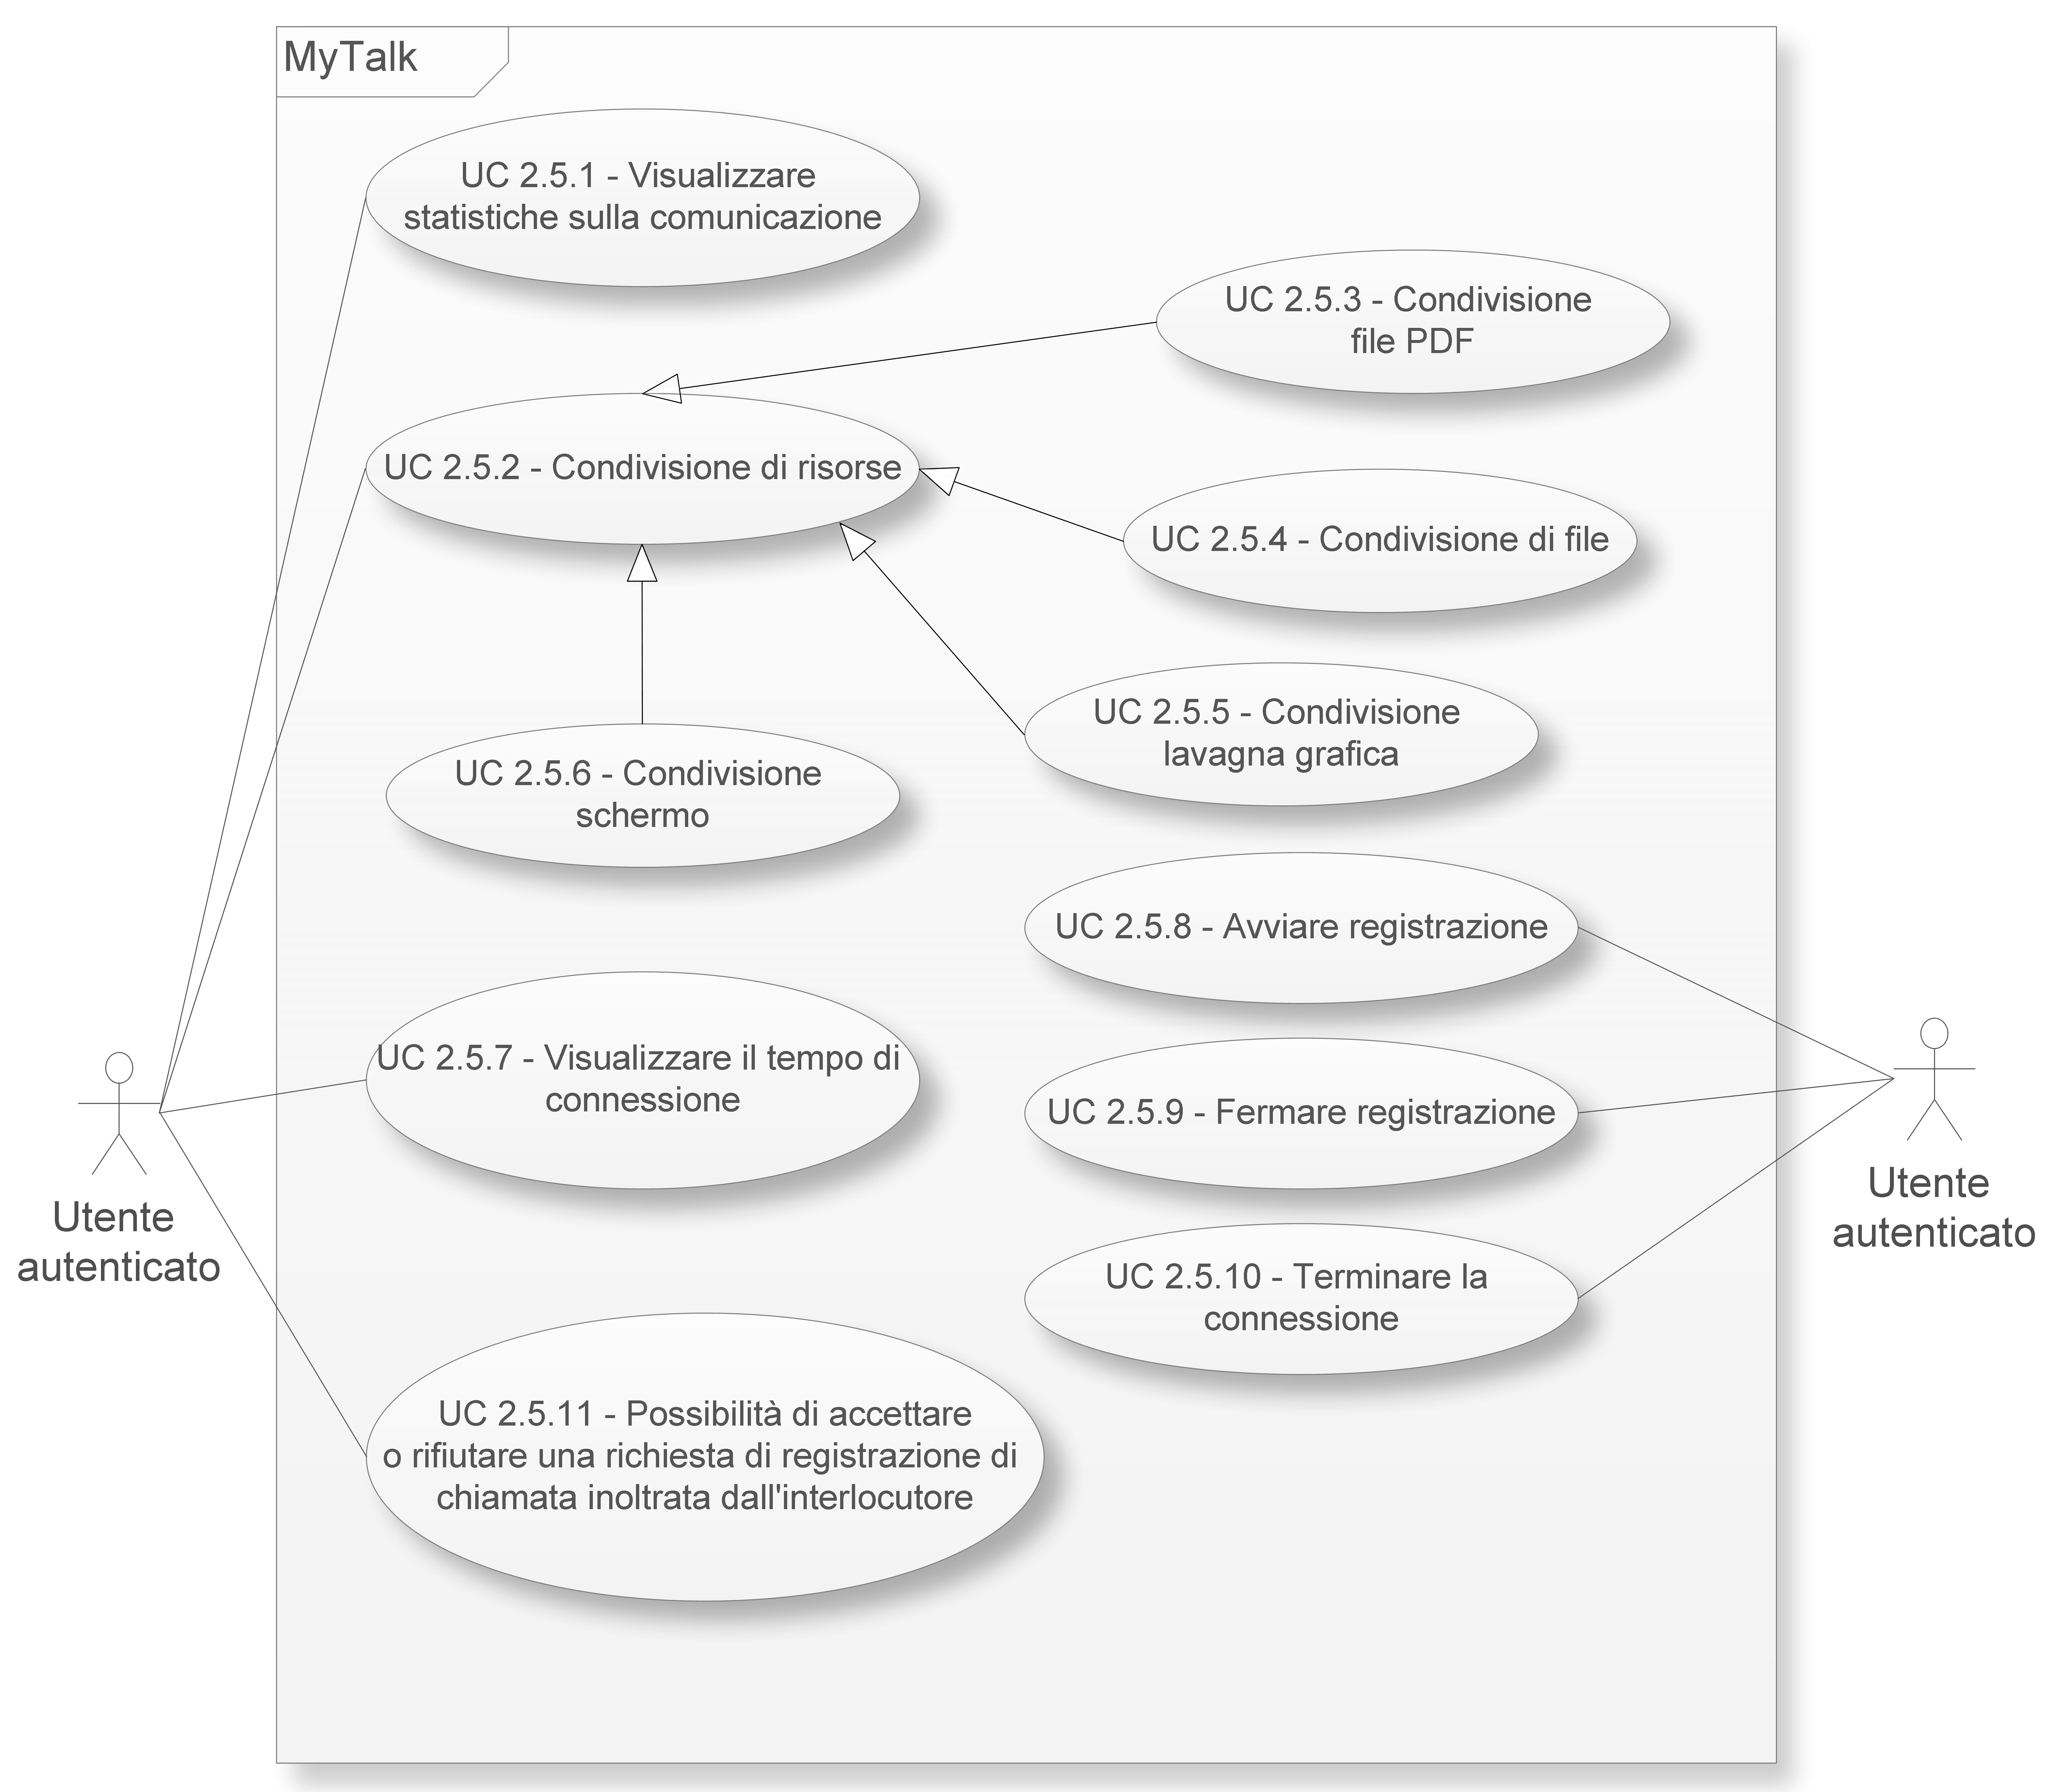
\includegraphics[width=.8\textwidth]{UC2-5}
\caption{UC2.5: Connessione con altri utenti autenticati}\label{fig:connessione}
\end{center}
\end{figure}
\begin{description}
\item{\scshape\bfseries Attori principali:}Utente autenticato.
\item{\scshape\bfseries Scopo e descrizione:} Un utente, durante una chiamata audio, audio/video e chat, può eseguire diverse operazioni sulla connessione stabilita.
\item{\scshape\bfseries Precondizione:} L'utente è autenticato nel sistema, ed ha già stabilito una connessione con un utente autenticato.
\item{\scshape\bfseries Postcondizione:} L'utente ha concluso la comunicazione. La causa della terminazione può essere attribuita alla chiusura volontaria della connessione oppure al fatto che l'utente rimane l'unico attivo nella connessione.
\item{\scshape\bfseries Illustrazione scenario principale:} L'utente ha avviato una comunicazione. Mentre questa è in esecuzione, l'utente potrà: visualizzare le statistiche sulla comunicazione (UC2.5.1), condividere delle risorse dal proprio dispositivo (Condivisione di PDF, invio di file, condivisione di una lavagna grafica, e condivisione dello schermo)(UC2.5.2), visualizzare da quanto tempo è aperta la connessione (UC2.5.3), avviare e fermare una registrazione (UC2.5.6 - UC2.5.7), accettare o rifiutare una richiesta di registrazione inoltrata da un interlocutore (UC2.5.4 - UC2.5.5). Infine l'utente può decidere di terminare la comunicazione (UC2.5.8).
\end{description}

\subsection{UC2.5.1: Visualizzazione statistiche sulla comunicazione}
\begin{figure}[H]
\begin{center}
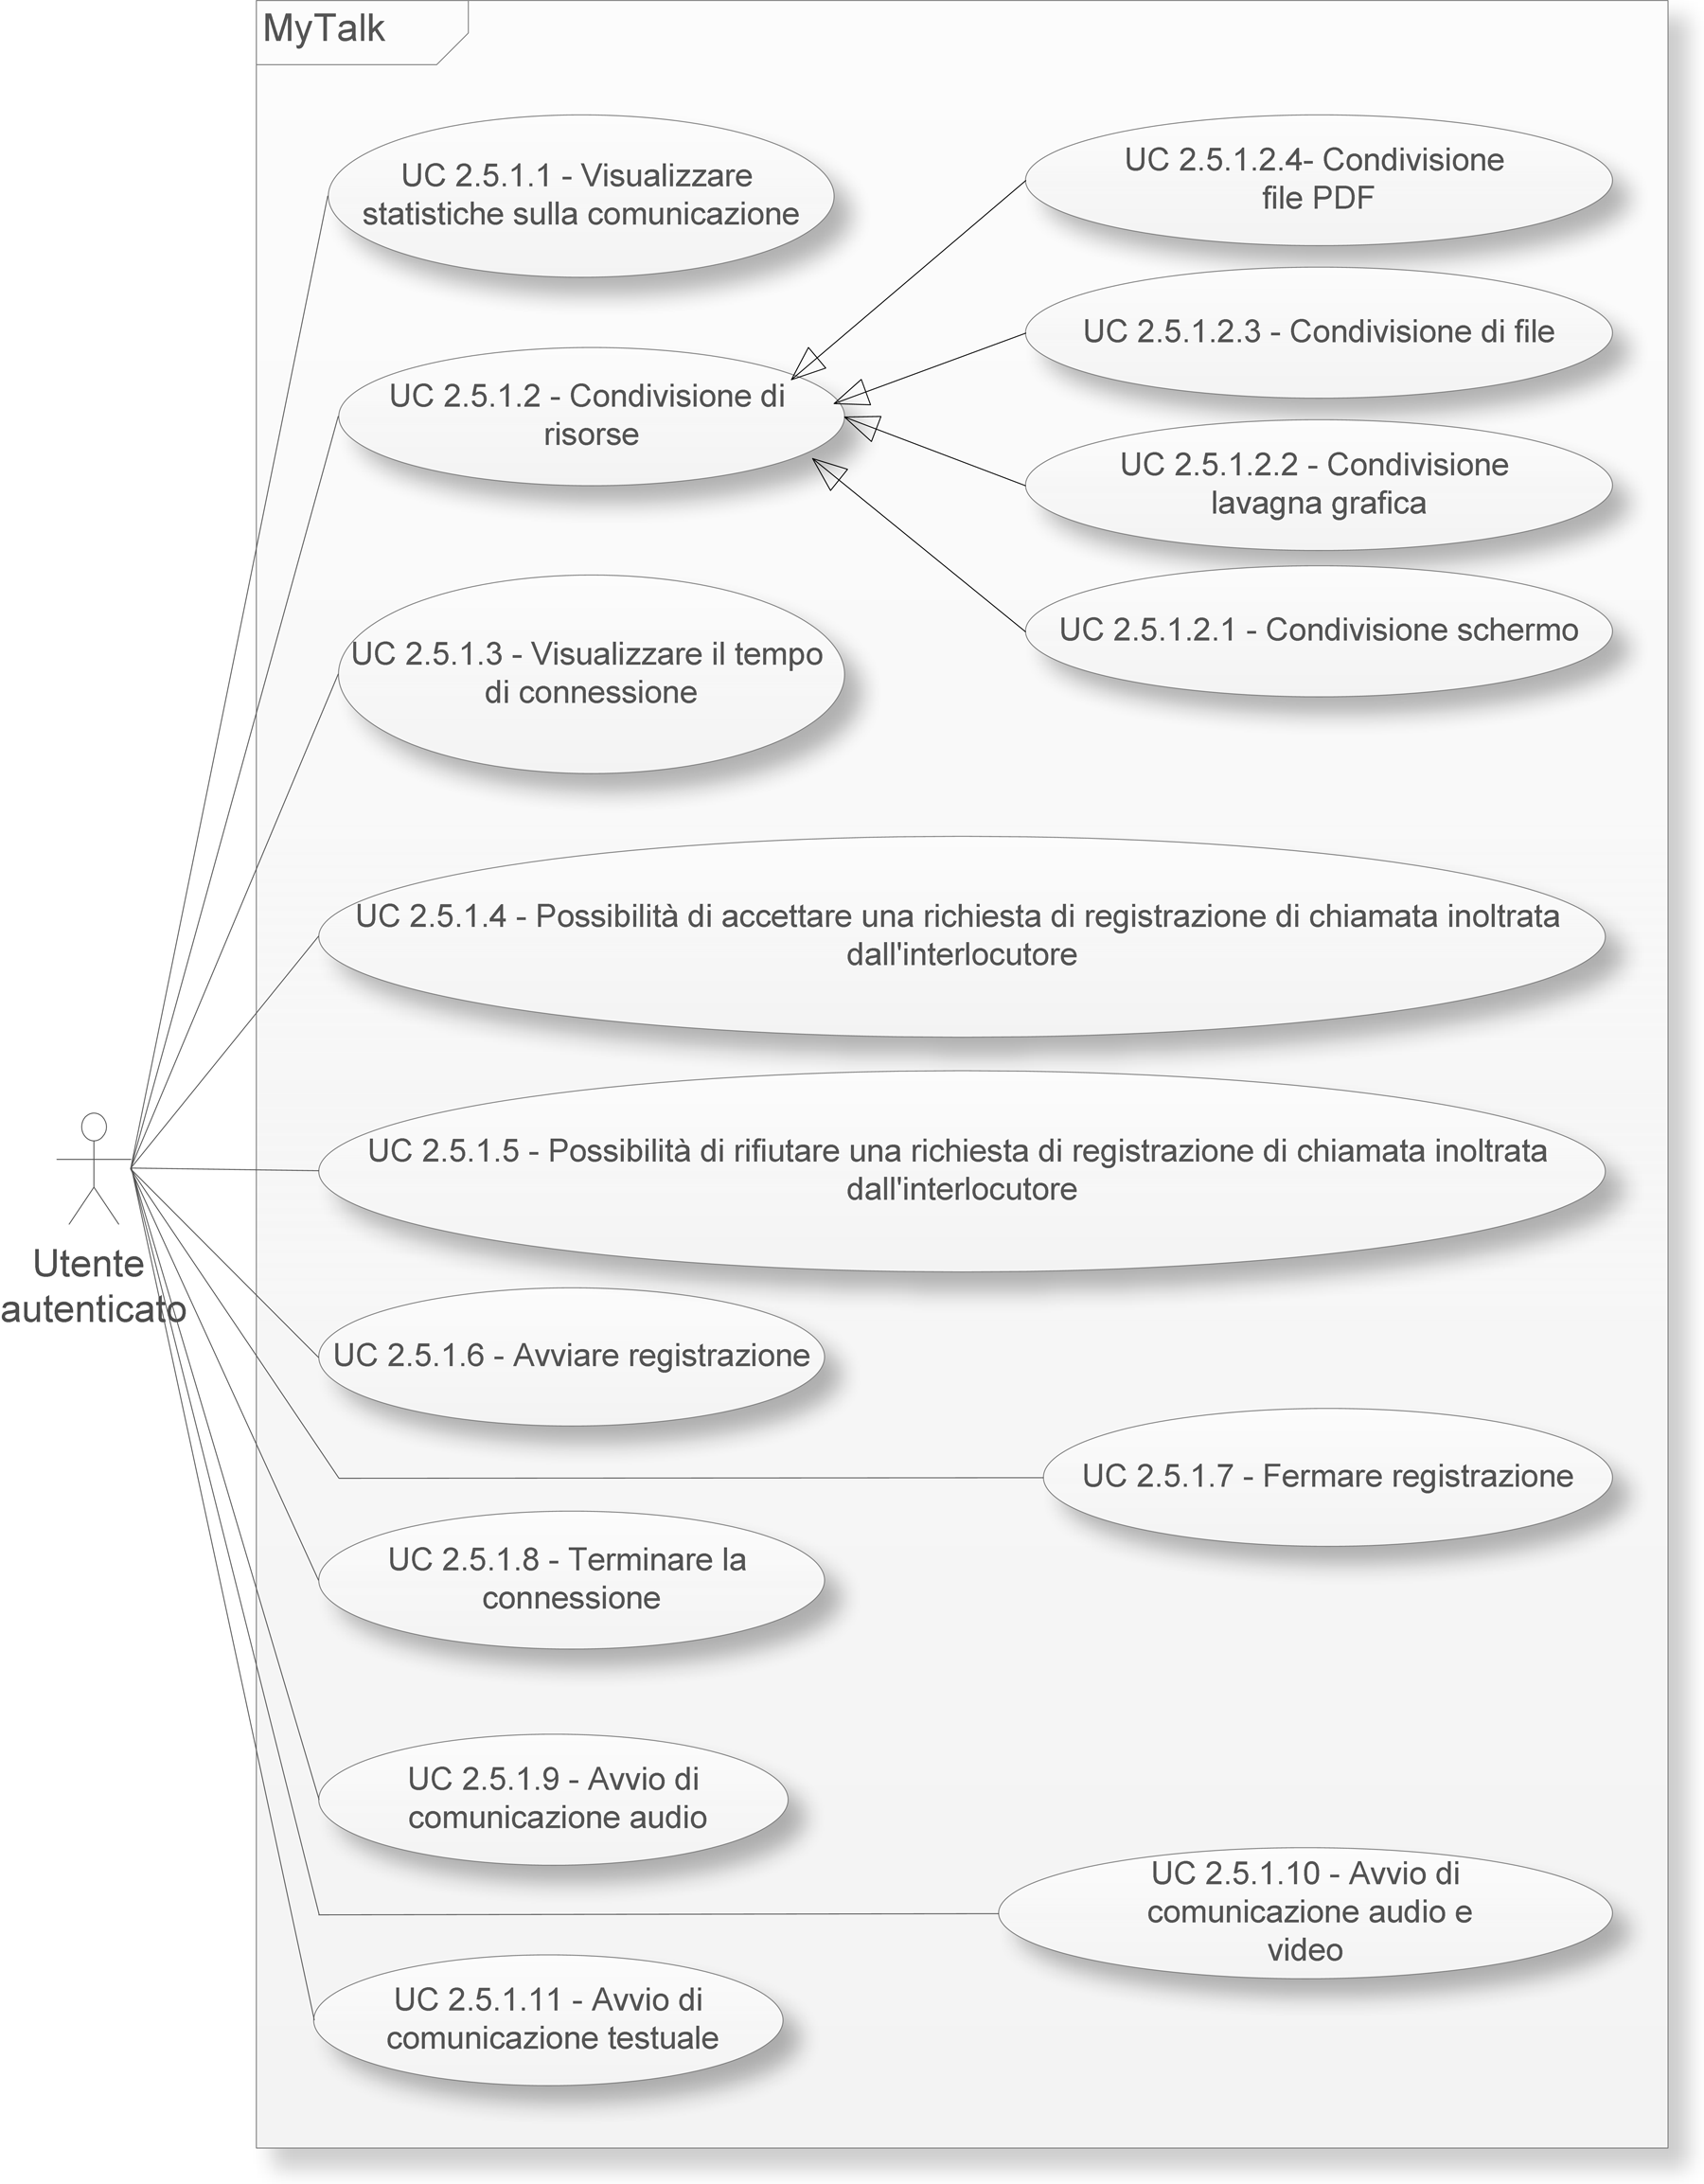
\includegraphics[width=.8\textwidth]{UC2-5-1}
\caption{UC2.5.1: Visualizzazione statistiche sulla comunicazione}\label{fig:visualizzazione_statistiche}
\end{center}
\end{figure}
\begin{description}
\item{\scshape\bfseries Attori principali:}Utente autenticato.
\item{\scshape\bfseries Scopo e descrizione:} L'utente visualizza i dettagli della comunicazione con un altro utente.
\item{\scshape\bfseries Precondizione:} L'utente sta comunicando con un altro utente del sistema.
\item{\scshape\bfseries Postcondizione:} L'utente ha visualizzato tutte le informazioni riguardanti la comunicazione.
\item{\scshape\bfseries Illustrazione scenario principale:} L'utente che comincia a comunicare con un altro utente ha a disposizione la visualizzazione di alcune informazioni sulla comunicazione in corso, come il numero di byte ricevuti ed inviati (UC2.5.1.2 - UC2.5.1.1), la latenza ossia il tempo che passa da quando un utente trasmette a quando l'altro utente riceve (UC2.5.1.3), la velocità di trasmissione dei dati (UC2.5.1.4) e i frame per secondo (fps) nel caso sia in corso una videochiamata (UC2.5.1.5).
\end{description}

\newpage\section{Requisiti di progetto}
I requisiti verranno suddivisi in base alla loro priorità. Rispettivamente seguirà la lista dei requisiti obbligatori, facoltativi e desiferabili. Ogni requisito è identificato con il seguente formato RXYZI con:


		\begin{itemize}

			\item \textbf{X}: indica la tipologia dell'utente interessato dal requisito. I possibili valori che X può assumere sono U (utente) oppure S (sistema).

			\item \textbf{Y}: indica la tipologia del requisito, e può assumere i valori: F(funzionale), Q(qualitativo), P(prestazionale), D(dichiarativo).

			\item \textbf{Z}: indica il livello di priorità del requisito. Può assumere i valori O(obbligatorio), \\F(facoltativo), D(desiderabile).

			\item \textbf{I}: indica l'id numerico del requisito, denominato secondo le direttive delle norme di progetto.

		\end{itemize}


		Ogni requisito si può suddividere in sottorequisiti. Tale evento è evidenziato dal valore del campo I, come riportato nelle norme di progetto. Infine i requisiti sono ordinati (nelle proprie sezioni) in base all'ordine crescente del campo numerico I.\
Per quanto riguarda invece i requisiti di processo, si rimanda ai documenti \textit{piano\_di\_qualifica.2.0.pdf} (sez. 3.1) e \textit{norme\_di\_progetto.2.0.pdf} (in particolare le sez. 2, 3 e 4).

\subsection{Requisiti funzionali}


\subsubsection{Requisiti funzionali obbligatori}

\begin{center}
\rowcolors{2}{lightblue}{llightblue}\begin{longtable}{lp{.55\textwidth}l}
\toprule Codice & Requisito & Fonte\\
\midrule
RUFO1.0.0 & L'utente deve potersi autentificare nel server, così da permettere a quest'ultimo di rilevare la sua presenza nel sistema. & Interno \\
RUFO2.0.0 & Registrazione del nuovo utente & Capitolato d'appalto \\
RUFO5.0.0 & Possibilità di visualizzare la lista di utenti registrati nel sistema & Capitolato d'appalto \\
RUFO6.1.0 & Stabilire e gestire una comunicazione audio con un utente in linea & Capitolato d'appalto \\
RUFO6.1.1 & Stabilire una comunicazione audio mediante inserimento d'indirizzo IP & Capitolato d'appalto \\
RUFO6.1.3 & Stabilire una comunicazione audio con un utente registrato e NON presente nella rubrica & Capitolato d'appalto \\
RUFO6.2.0 & Stabilire e gestire  una comunicazione audio e video con un utente & Capitolato d'appalto \\
RUFO6.2.1 & Stabilire una comunicazione audio e video mediante inserimento d'indirizzo IP & Capitolato d'appalto \\
RUFO6.2.3 & Stabilire una comunicazione audio e video con un utente registrato e NON presente nella rubrica & Capitolato d'appalto \\
RUFO7.0.0 & Indicare il tempo di comunicazione & Capitolato d'appalto \\
RUFO8.0.0 & Valutare il numero di byte trasmessi & Capitolato d'appalto \\
RUFO8.1.0 & Valutare il numero di byte inviati & Interno \\
RUFO8.2.0 & Valutare il numero di byte ricevuti & Interno \\
RUFO9.0.0 & Indicare la qualità della linea di trasmissione & Capitolato d'appalto \\
RUFO9.1.0 & Rilevare latenza & Capitolato d'appalto \\
RUFO9.2.0 & Rilevare velocità di trasmissione & Capitolato d'appalto \\
RSFO11.0.0 & Creare una connessione tra client, mediante l'utilizzo di un server & Capitolato d'appalto \\
RSFO11.1.0 & Utilizzo del protocollo webSocket per creare una connessione tra 2 utenti & Interno \\
RSFO12.0.0 & Gestire gli eventi dell'utente durante la connessione. & Interno \\
RUFO12.3.0 & Chi partecipa alla connessione può togliersi da essa & Interno \\
\bottomrule
\end{longtable}
\end{center}

\subsubsection{Requisiti funzionali desiderabili}

\begin{center}
\rowcolors{2}{lightblue}{llightblue}\begin{longtable}{lp{.55\textwidth}l}
\toprule Codice & Requisito & Fonte\\
\midrule
RUFD1.1.0 & Gestione password dimenticata & Interno \\
RUFD1.1.1 & Proporre la domanda segreta all'utente & Interno \\
RUFD1.1.2 & Invio di una mail all'utente contenete la password dimenticata & Interno \\
RUFD12.2.0 & Chi crea la connessione può eliminare i membri del gruppo & Interno \\
RUFD13.1.0 & Servizio chat tra 2 utenti & Interno \\
\bottomrule
\end{longtable}
\end{center}

\subsubsection{Requisiti funzionali facoltativi}

\begin{center}
\rowcolors{2}{lightblue}{llightblue}\begin{longtable}{lp{.55\textwidth}l}
\toprule Codice & Requisito & Fonte\\
\midrule
RUFF3.0.0 & Modifica dati utente (ad eccezione dell'indirizzo email) & Interno \\
RUFF3.1.0 & Modifica dei dati per l'autenticazione quali password, domanda segreta e risposta alla domanda segreta (l'e-mail non può essere modificata) & Interno \\
RUFF3.2.0 & Modifica dei dati anagrafici facoltativi quali nome, cognome e immagine del profilo & Interno \\
RUFF4.0.0 & L'utente dovrebbe poter tenere una rubrica personale dove raggruppare i propri contatti. & Interno \\
RUFF4.1.0 & Un utente deve poter inserire utenti nella propria rubrica. & Capitolato d'appalto \\
RUFF4.2.0 & Eliminare un utente dalla propria rubrica & Interno \\
RUFF4.3.0 & Possibilità di ordinare la rubrica su alcuni parametri rilevanti & Interno \\
RUFF4.4.0 & Possibilità di suddividere la rubrica in gruppi & Interno \\
RUFF4.4.1 & Possibilità di togliere un elemento da un gruppo & Interno \\
RUFF4.4.2 & Possibilità di aggiungere un elemento in un gruppo & Interno \\
RUFF4.4.3 & Possibilità di creare un gruppo & Interno \\
RUFF4.4.4 & Possibilità di eliminare un gruppo & Interno \\
RUFF4.5.0 & Possibilità di esportare in xml la rubrica personale & Interno \\
RUFF4.6.0 & Possibilità di modificare la rubrica importando un file xml & Interno \\
RUFF4.7.0 & Ricerca di un utente nella propria rubrica. & Interno \\
RUFF5.1.0 & Possibilità di cercare un utente dalla lista & Interno \\
RUFF6.1.2 & Stabilire una comunicazione audio con un utente registrato e presente nella rubrica & Capitolato d'appalto \\
RUFF6.1.4 & Promuovere una comunicazione audio avviata con un utente in una comunicazione audio e video & Interno \\
RUFF6.2.2 & Stabilire una comunicazione audio e video con un utente registrato e presente nella rubrica & Capitolato d'appalto \\
RUFF6.2.4 & Declassare una comunicazione audio e video avviata con un utente in una comunicazione solo audio & Interno \\
RUFF6.2.5 & Disattivare la webcam utente pur continuando a ricevere il segnale video proveniente dall'altro capo della comunicazione & Interno \\
RUFF6.3.0 & Disattivare il microfono utente pur continuando a ricevere il segnale video proveniente dall'altro capo della comunicazione & Interno \\
RUFF9.3.0 & Rilevazione frame per secondo & Interno \\
RSFF11.2.0 & Utilizzo del protocollo webSocket per creare una connessione tra più di 2 utenti & Interno \\
RSFF12.1.0 & Estendere la connessione ad altri client & Interno \\
RUFF13.0.0 & Servizio chat testuale & Capitolato d'appalto \\
RUFF13.2.0 & Servizio chat tra più di 2 utenti & Interno \\
RUFF14.0.0 & Registrazione della chiamata & Capitolato d'appalto \\
RUFF14.1.0 & Necessità di autorizzazione dagli utenti della chiamata per poter avviare la registrazione & Interno \\
RUFF14.2.0 & Registrazione audio & Interno \\
RUFF14.3.0 & Possibilità di riascoltare la registrazione & Interno \\
RUFF15.0.0 & L'utente avrà a disposizione una segreteria telefonica. & Interno \\
RUFF15.1.0 & Possibilità di lasciare un audio messaggio in segreteria & Interno \\
RUFF15.2.0 & Possibilità di lasciare un audio e video messaggio in segreteria & Capitolato d'appalto \\
RUFF15.3.0 & Possibilità di ascoltare la propria segreteria & Interno \\
RUFF15.4.0 & Possibilità di cancellare messaggi della segretaria & Interno \\
RUFF15.5.0 & Possibilità di cambiare lo stato del messaggio tra ascoltato/non ascoltato & Interno \\
RUFF16.0.0 & Possibilità di impostare lo stato utente: disponibile o non disponibile & Interno \\
RUFF17.0.0 & Dare la possibilità di vedere gli stati personali altrui. & Interno \\
RUFF18.0.0 & Creazione di una Blacklist & Interno \\
RUFF19.0.0 & Possibilità di tenere uno storico delle chiamate & Interno \\
RUFF20.0.0 & Condividere risorse & Interno \\
RUFF20.1.0 & Condividere monitor & Interno \\
RUFF20.2.0 & Condivisione pdf & Interno \\
RUFF20.3.0 & Condivisione lavagna grafica. & Interno \\
RUFF20.4.0 & Invio file & Interno \\
\bottomrule
\end{longtable}
\end{center}


\subsection{Requisiti qualitativi}

\subsubsection{Requisiti qualitativi obbligatori}

\begin{center}
\rowcolors{2}{lightblue}{llightblue}\begin{longtable}{lp{.55\textwidth}l}
\toprule Codice & Requisito & Fonte\\
\midrule
RSQO1.2.0 & Il Login avviene tramite l'inserimento di username (e-mail) e password & Interno \\
RSQO2.1.0 & Inserimento dei dati obbligatori per l'autenticazione quali username (e-mail), password, domanda segreta e risposta alla domanda segreta & Interno \\
RSDO6.4.0 & L'applicativo dev'essere predisposto a facili modifiche dettate da evoluzioni future di WebRTC. & Capitolato d'appalto \\
\bottomrule
\end{longtable}
\end{center}

\subsubsection{Requisiti qualitativi desiderabili}

\begin{center}
\rowcolors{2}{lightblue}{llightblue}\begin{longtable}{lp{.55\textwidth}l}
\toprule Codice & Requisito & Fonte\\
\midrule
RSQD2.1.1 & L'utente ha una stima per la complessità della propria password & Interno \\
RSQD2.1.2 & Convalidare username (e-mail) dell'utente & Interno \\
RSQD21.0.0 & Gestione interfaccia grafica in più lingue & Interno \\
\bottomrule
\end{longtable}
\end{center}

\subsubsection{Requisiti qualitativi facoltativi}

\begin{center}
\rowcolors{2}{lightblue}{llightblue}\begin{longtable}{lp{.55\textwidth}l}
\toprule Codice & Requisito & Fonte\\
\midrule
RSQF23.0.0 & Verificare che l'applicativo funzioni anche sotto gli altri browser del S.O. Windows & Interno \\
RSQF23.1.0 & Verificare che funzioni con Opera (versione 12.0 minima) & Capitolato d'appalto \\
RSQF23.2.0 & Verificare che funzioni con Firefox (versione 17.0 minima) & Capitolato d'appalto \\
RSQF23.3.0 & Verificare che funzioni con Internet Explorer (versione 10.0 minima) & Capitolato d'appalto \\
RSQF23.4.0 & Verificare che funzioni con Safari (versione 6.0 minima) & Capitolato d'appalto \\
RSQF24.0.0 & Verificare che l'applicativo funzioni anche sotto gli altri browser del S.O. Linux & Interno \\
RSQF24.1.0 & Verificare che funzioni con Opera (versione 12.0 minima) & Capitolato d'appalto \\
RSQF24.2.0 & Verificare che funzioni con Firefox (versione 17.0 minima) & Capitolato d'appalto \\
RSQF24.3.0 & Verificare che funzioni con Chromium (versione 25.0.1313 minima) & Interno \\
RSQF25.0.0 & Verificare che l'applicativo funzioni anche sotto gli altri browser del S.O. Macintosh & Interno \\
RSQF25.1.0 & Verificare che funzioni con Opera (versione 12.0 minima) & Capitolato d'appalto \\
RSQF25.2.0 & Verificare che funzioni con Firefox (versione 17.0 minima) & Capitolato d'appalto \\
RSQF25.3.0 & Verificare che funzioni con Safari  (versione 6.0 minima) & Capitolato d'appalto \\
RSQF26.0.0 & Il software dovrà essere compatibile con componenti realizzati in Flash & Capitolato d'appalto \\
\bottomrule
\end{longtable}
\end{center}

\subsection{Requisiti dichiarativi}

\subsubsection{Requisiti dichiarativi obbligatori}

\begin{center}
\rowcolors{2}{lightblue}{llightblue}\begin{longtable}{lp{.55\textwidth}l}
\toprule Codice & Requisito & Fonte\\
\midrule
RSDO6.0.0 & Gestire le comunicazioni utente tramite WebRTC & Capitolato d'appalto \\
RSDO10.0.0 & L'intero sistema deve essere contenuto in un unica pagina Web & Capitolato d'appalto \\
RSDO10.1.0 & L'interfaccia grafica non deve subire refresh per ogni operazione dell'utente & Interno \\
RSDO11.3.0 & Il server sarà implementato tramite il linguaggio Java. & Capitolato d'appalto \\
RSDO11.4.0 & Il server non sarà coinvolto nella comunicazione tra due o più utenti se non per avviare una comunicazione. & Capitolato d'appalto \\
RSDO22.0.0 & L'applicativo deve essere fruibile attraverso un browser web &  \\
RSDO22.1.0 & L'applicativo web deve funzionare nel browser web Google Chrome (versione minima 23.0.1271.97m) & Capitolato d'appalto \\
\bottomrule
\end{longtable}
\end{center}

\newpage\section{Tracciamento use case - requisiti}\label{sec:tracciamento}

\begin{center}
\rowcolors{2}{lightblue}{llightblue}\begin{longtable}{lp{.55\textwidth}l}
\toprule Codice UC & Nome UC  & Requisito\\
\midrule
UC1 & Login e registrazione & RUFO1.0.0 \\
 &  & RUFD1.1.0 \\
 &  & RUFD1.1.1 \\
 &  & RUFD1.1.2 \\
 &  & RSQO1.2.0 \\
 &  & RUFO2.0.0 \\
 &  & RSQO2.1.0 \\
 &  & RSQD2.1.1 \\
 &  & RSQD2.1.2 \\
 &  & RSDD2.2.0 \\
UC2 & Home screen dell'applicativo & RUFF3.0.0 \\
 &  & RUFF3.1.0 \\
 &  & RUFF3.2.0 \\
 &  & RUFF4.0.0 \\
 &  & RUFF4.1.0 \\
 &  & RUFF4.2.0 \\
 &  & RUFF4.3.0 \\
 &  & RUFF4.4.0 \\
 &  & RUFF4.4.1 \\
 &  & RUFF4.4.2 \\
 &  & RUFF4.4.3 \\
 &  & RUFF4.4.4 \\
 &  & RUFF4.5.0 \\
 &  & RUFF4.6.0 \\
 &  & RUFF4.7.0 \\
 &  & RUFO5.0.0 \\
 &  & RUFF5.1.0 \\
 &  & RUFO6.1.0 \\
 &  & RUFO6.1.1 \\
 &  & RUFF6.1.2 \\
 &  & RUFO6.1.3 \\
 &  & RUFF6.1.4 \\
 &  & RUFO6.2.0 \\
 &  & RUFO6.2.1 \\
 &  & RUFF6.2.2 \\
 &  & RUFO6.2.3 \\
 &  & RUFF6.2.4 \\
 &  & RUFF6.2.5 \\
 &  & RUFF6.3.0 \\
 &  & RUFO7.0.0 \\
 &  & RUFO8.0.0 \\
 &  & RUFO8.1.0 \\
 &  & RUFO8.2.0 \\
 &  & RUFO9.0.0 \\
 &  & RUFO9.1.0 \\
 &  & RUFO9.2.0 \\
 &  & RUFF9.3.0 \\
 &  & RSFF12.1.0 \\
 &  & RUFD12.2.0 \\
 &  & RUFO12.3.0 \\
 &  & RUFF13.0.0 \\
 &  & RUFD13.1.0 \\
 &  & RUFF13.2.0 \\
 &  & RUFF14.0.0 \\
 &  & RUFF14.1.0 \\
 &  & RUFF14.2.0 \\
 &  & RUFF15.0.0 \\
 &  & RUFF15.1.0 \\
 &  & RUFF15.2.0 \\
 &  & RUFF15.3.0 \\
 &  & RUFF15.4.0 \\
 &  & RUFF15.5.0 \\
 &  & RUFF16.0.0 \\
 &  & RUFF17.0.0 \\
 &  & RUFF18.0.0 \\
 &  & RUFF19.0.0 \\
 &  & RUFF20.0.0 \\
 &  & RUFF20.1.0 \\
 &  & RUFF20.2.0 \\
 &  & RUFF20.3.0 \\
 &  & RUFF20.4.0 \\
UC1.1 & Login utente & RUFO1.0.0 \\
 &  & RSQO1.2.0 \\
UC1.2 & Registrazione & RUFO2.0.0 \\
 &  & RSQO2.1.0 \\
 &  & RSQD2.1.1 \\
 &  & RSQD2.1.2 \\
 &  & RSDD2.2.0 \\
UC1.3 & Recupero della password & RUFD1.1.0 \\
 &  & RUFD1.1.1 \\
 &  & RUFD1.1.2 \\
UC2.1 & Gestione account & RUFF3.0.0 \\
 &  & RUFF3.1.0 \\
 &  & RUFF3.2.0 \\
UC2.2 & Gestire lo stato & RUFF16.0.0 \\
UC2.3 & Gestione della rubrica & RUFF4.0.0 \\
 &  & RUFF4.1.0 \\
 &  & RUFF4.2.0 \\
 &  & RUFF4.3.0 \\
 &  & RUFF4.4.0 \\
 &  & RUFF4.4.1 \\
 &  & RUFF4.4.2 \\
 &  & RUFF4.4.3 \\
 &  & RUFF4.4.4 \\
 &  & RUFF4.5.0 \\
 &  & RUFF4.6.0 \\
 &  & RUFF4.7.0 \\
 &  & RUFO5.0.0 \\
 &  & RUFF5.1.0 \\
 &  & RUFF18.0.0 \\
UC2.4 & Gestire segreteria personale & RUFF15.0.0 \\
 &  & RUFF15.1.0 \\
 &  & RUFF15.2.0 \\
 &  & RUFF15.3.0 \\
 &  & RUFF15.4.0 \\
 &  & RUFF15.5.0 \\
UC2.5 & Connessione con altri utenti autenticati & RUFO6.1.0 \\
 &  & RUFO6.1.1 \\
 &  & RUFF6.1.2 \\
 &  & RUFO6.1.3 \\
 &  & RUFF6.1.4 \\
 &  & RUFO6.2.0 \\
 &  & RUFO6.2.1 \\
 &  & RUFF6.2.2 \\
 &  & RUFO6.2.3 \\
 &  & RUFF6.2.4 \\
 &  & RUFF6.2.5 \\
 &  & RUFF6.3.0 \\
 &  & RUFO7.0.0 \\
 &  & RUFO8.0.0 \\
 &  & RUFO8.1.0 \\
 &  & RUFO8.2.0 \\
 &  & RUFO9.0.0 \\
 &  & RUFO9.1.0 \\
 &  & RUFO9.2.0 \\
 &  & RUFF9.3.0 \\
 &  & RSFO12.0.0 \\
 &  & RSFF12.1.0 \\
 &  & RUFD12.2.0 \\
 &  & RUFO12.3.0 \\
 &  & RUFF13.0.0 \\
 &  & RUFD13.1.0 \\
 &  & RUFF13.2.0 \\
 &  & RUFF14.0.0 \\
 &  & RUFF14.1.0 \\
 &  & RUFF14.2.0 \\
 &  & RUFF20.0.0 \\
 &  & RUFF20.1.0 \\
 &  & RUFF20.2.0 \\
 &  & RUFF20.3.0 \\
 &  & RUFF20.4.0 \\
UC2.3.1 & Aggiungi contatto & RUFF4.1.0 \\
UC2.5.1 & Visualizzazione statistiche sulla comunicazione & RUFO7.0.0 \\
 &  & RUFO8.0.0 \\
 &  & RUFO8.1.0 \\
 &  & RUFO8.2.0 \\
 &  & RUFO9.0.0 \\
 &  & RUFO9.1.0 \\
 &  & RUFO9.2.0 \\
 &  & RUFF9.3.0 \\
\bottomrule
\end{longtable}
\end{center}
\newpage\section{Tracciamento requisiti - use case}\label{sec:tracciamento}

\begin{center}
\rowcolors{2}{lightblue}{llightblue}\begin{longtable}{lp{.55\textwidth}l}
\toprule Requisito & Codice UC\\
\midrule
RUFO1.0.0 & UC1 \\
 & UC1.1 \\
RUFD1.1.0 & UC1 \\
 & UC1.3 \\
RUFD1.1.1 & UC1 \\
 & UC1.3 \\
RUFD1.1.2 & UC1 \\
 & UC1.3 \\
RSQO1.2.0 & UC1 \\
 & UC1.1 \\
RUFO2.0.0 & UC1 \\
 & UC1.2 \\
RSQO2.1.0 & UC1 \\
 & UC1.2 \\
RSQD2.1.1 & UC1 \\
 & UC1.2 \\
RSQD2.1.2 & UC1 \\
 & UC1.2 \\
RSDD2.2.0 & UC1 \\
 & UC1.2 \\
RUFF3.0.0 & UC2 \\
 & UC2.1 \\
RUFF3.1.0 & UC2 \\
 & UC2.1 \\
RUFF3.2.0 & UC2 \\
 & UC2.1 \\
RUFF4.0.0 & UC2 \\
 & UC2.3 \\
RUFF4.1.0 & UC2 \\
 & UC2.3 \\
 & UC2.3.1 \\
RUFF4.2.0 & UC2 \\
 & UC2.3 \\
RUFF4.3.0 & UC2 \\
 & UC2.3 \\
RUFF4.4.0 & UC2 \\
 & UC2.3 \\
RUFF4.4.1 & UC2 \\
 & UC2.3 \\
RUFF4.4.2 & UC2 \\
 & UC2.3 \\
RUFF4.4.3 & UC2 \\
 & UC2.3 \\
RUFF4.4.4 & UC2 \\
 & UC2.3 \\
RUFF4.5.0 & UC2 \\
 & UC2.3 \\
RUFF4.6.0 & UC2 \\
 & UC2.3 \\
RUFF4.7.0 & UC2 \\
 & UC2.3 \\
RUFO5.0.0 & UC2 \\
 & UC2.3 \\
RUFF5.1.0 & UC2 \\
 & UC2.3 \\
RUFO6.1.0 & UC2 \\
 & UC2.5 \\
RUFO6.1.1 & UC2 \\
 & UC2.5 \\
RUFF6.1.2 & UC2 \\
 & UC2.5 \\
RUFO6.1.3 & UC2 \\
 & UC2.5 \\
RUFF6.1.4 & UC2 \\
 & UC2.5 \\
RUFO6.2.0 & UC2 \\
 & UC2.5 \\
RUFO6.2.1 & UC2 \\
 & UC2.5 \\
RUFF6.2.2 & UC2 \\
 & UC2.5 \\
RUFO6.2.3 & UC2 \\
 & UC2.5 \\
RUFF6.2.4 & UC2 \\
 & UC2.5 \\
RUFF6.2.5 & UC2 \\
 & UC2.5 \\
RUFF6.3.0 & UC2 \\
 & UC2.5 \\
RUFO7.0.0 & UC2 \\
 & UC2.5 \\
 & UC2.5.1 \\
RUFO8.0.0 & UC2 \\
 & UC2.5 \\
 & UC2.5.1 \\
RUFO8.1.0 & UC2 \\
 & UC2.5 \\
 & UC2.5.1 \\
RUFO8.2.0 & UC2 \\
 & UC2.5 \\
 & UC2.5.1 \\
RUFO9.0.0 & UC2 \\
 & UC2.5 \\
 & UC2.5.1 \\
RUFO9.1.0 & UC2 \\
 & UC2.5 \\
 & UC2.5.1 \\
RUFO9.2.0 & UC2 \\
 & UC2.5 \\
 & UC2.5.1 \\
RUFF9.3.0 & UC2 \\
 & UC2.5 \\
 & UC2.5.1 \\
RSFO12.0.0 & UC2.5 \\
RSFF12.1.0 & UC2 \\
 & UC2.5 \\
RUFD12.2.0 & UC2 \\
 & UC2.5 \\
RUFO12.3.0 & UC2 \\
 & UC2.5 \\
RUFF13.0.0 & UC2 \\
 & UC2.5 \\
RUFD13.1.0 & UC2 \\
 & UC2.5 \\
RUFF13.2.0 & UC2 \\
 & UC2.5 \\
RUFF14.0.0 & UC2 \\
 & UC2.5 \\
RUFF14.1.0 & UC2 \\
 & UC2.5 \\
RUFF14.2.0 & UC2 \\
 & UC2.5 \\
RUFF15.0.0 & UC2 \\
 & UC2.4 \\
RUFF15.1.0 & UC2 \\
 & UC2.4 \\
RUFF15.2.0 & UC2 \\
 & UC2.4 \\
RUFF15.3.0 & UC2 \\
 & UC2.4 \\
RUFF15.4.0 & UC2 \\
 & UC2.4 \\
RUFF15.5.0 & UC2 \\
 & UC2.4 \\
RUFF16.0.0 & UC2 \\
 & UC2.2 \\
RUFF17.0.0 & UC2 \\
RUFF18.0.0 & UC2 \\
 & UC2.3 \\
RUFF19.0.0 & UC2 \\
RUFF20.0.0 & UC2 \\
 & UC2.5 \\
RUFF20.1.0 & UC2 \\
 & UC2.5 \\
RUFF20.2.0 & UC2 \\
 & UC2.5 \\
RUFF20.3.0 & UC2 \\
 & UC2.5 \\
RUFF20.4.0 & UC2 \\
 & UC2.5 \\
\bottomrule
\end{longtable}
\end{center}
